% ***************************************************************************************************
%
%	Szablon pracy magisterskiej dla Politechniki Wrocławskiej w wersji dwustronnej.
%	Autor:	Tomasz Strzałka
%
% ***************************************************************************************************

% Styl dwustronny z domyślną wielkością czcionki 10pt oraz oddzieloną stroną tytułową (titlepage).
% Domyślnie rodziały rozpoczynają się na stronie prawej (openright).
\documentclass[a4paper,11pt,twoside,openright]{book}
% \RequirePackage{luatex85,shellesc}
\usepackage{luatex85}
\usepackage{shellesc}

\renewcommand{\baselinestretch}{1.2} 

% ***************************************************************************************************
% Ustawienia języka
% ***************************************************************************************************

% Podstawowe ustawienia języka, według którego formatowany będzie dokument
\usepackage[english]{babel}
\usepackage{csquotes}
% Pakiet babel dla polskiego języka powoduje konflikt z pakietem amssymb.
% Polecenie '\lll' definiują oba pakiety - porządana jest druga definicja.

% W przypadku wielojęzykowości ustawia główny język dokumentu
\selectlanguage{english}

% Kodowanie dokumentu
% \usepackage[utf8]{inputenc}

% Dowolny rozmiar czcionek, kodowanie znaków
\usepackage{lmodern}

% Polskie wcięcia akapitów
% \usepackage{indentfirst}

% Polskie łamanie wyrazów
% \usepackage[plmath]{english}

% Przecinek w wyrażeniach matematycznych zamiast kropki
% \usepackage{icomma}

% Polskie formatowanie typograficzne
% \frenchspacing

% Zapewnia liczne usprawnienia wyświetlania i organizacji matematycznych formuł. 
\usepackage{amsmath}

% Wprowadza rozszerzony zestaw symboli m.in. \leadsto
\usepackage{amssymb}

% Dodatkowa, ,,kręcona'' czcionka matematyczna
\usepackage{mathrsfs}

% Dodatkowe wsparcie dla środowiska mathbb, które nie wspiera domyślnie cyfr (\mathbb{})
\usepackage{bbold}


% Fixes/improves amsmath
\usepackage{mathtools}


% ***************************************************************************************************
% Kolory  
% ***************************************************************************************************

% Umożliwia kolorowanie poszczególnych komórek tabeli
\usepackage[table]{xcolor}% http://ctan.org/pkg/

% Umożliwia łatwą zmianę koloru linii w tabeli
\usepackage{tabu}

% Umożliwia rozszerzoną kontrolę nad kolorami.
\usepackage{xcolor}

% Definicje kolorów
\definecolor{lgray}{HTML}{9F9F9F}
\definecolor{dgray}{HTML}{5F5F5F}
% lgray				-	nazwa nowo zdefiniowanego koloru
% HTML				-	model kolorów
% CCCCCC			-	wartość koloru zgodna z modelem

% ***************************************************************************************************
% Algorytmy 
% ***************************************************************************************************

% Udostępnia środowisko do konstruowania pseudokodów
% \usepackage[ruled,vlined,linesnumbered,longend,algochapter]{algorithm2e}
% ruled	- poziome kreski na początku i końcu algorytmu, podpis na górze oddzielony również kreską poziomą
% vlined - pionowe kreski łączące początek polecenia z jego końcem
% linesnumbered	- numerowanie kolejnych wierszy algorytmu
% longend - długie końcówki np. ifend, forend itd.
% algochapter - numeracja z rozdziałami

% Zmiana rozmiaru komentarzy
% \newcommand\algcomment[1]{
	% \footnotesize{#1}
% }

% Ustawienie zadanego stylu dla komentarzy
% \SetCommentSty{algcomment}


% \usepackage{newtxtext}
% \usepackage{newtxmath}

% Wyśrodkowana tylda
\usepackage{textcomp}%
\newcommand{\textapprox}{\raisebox{0.5ex}{\texttildelow}}

% Listowanie kodów źródłowych
\usepackage{listings} 

% ***************************************************************************************************
% Marginesy 
% ***************************************************************************************************

% Ustawienia rozmiarów stron i ich marginesów
\usepackage[headheight=18pt, top=25mm, bottom=25mm, left=25mm, right=25mm, bindingoffset=5mm]{geometry}
% headheight		-	wysokość tytułów
% top				-	margines górny
% bottom			-	margines dolny
% left				-	margines lewy
% right				-	margines prawy

% Usunięcie górnego marginesu dla środowisk
\makeatletter
\setlength\@fptop{0\p@}	
\makeatother

% ***************************************************************************************************
% Styl 
% ***************************************************************************************************

% Definiuje środowisko 'titlingpage', które zapewnia pełną kontrolę nad układem strony tytułowej.
\usepackage{titling}


% Umożliwia modyfikowanie stylu spisu treści
\usepackage{tocloft}	

\tocloftpagestyle{tableOfContentStyle}

% Definiowanie własnych stylów nagłówków i/lub stopek
\usepackage{fancyhdr}

% Domyślny styl dla pracy 
\fancypagestyle{custom}{
	\fancyhf{}									% wyczyść stopki i nagłówki
	\fancyhead[RO]{								% Prawy, nieparzysty nagłówek
		\hrulefill \hspace{16pt} \large Chapter \thechapter
		\put(-455.4, 13.5){%
			\makebox(0,0)[l]{%
				
\includegraphics[width=0.05\textwidth]{Figures/pwr-logo}
			}
		}
		\put(-426,5.5){%
			\makebox(0,0)[l]{%
				\small Wrocław University of Science and Technology
			}
		}
	}
	\fancyhead[LE]{								% Lewy, parzysty nagłówek
		\large Chapter \thechapter \hspace{16pt} \hrulefill 
		\put(-20, 12.1){%
			\makebox(0,0)[l]{%
				
\includegraphics[width=0.05\textwidth]{Figures/wppt-logo}
			}
		}
		\put(-240,5.5){%
			\makebox(0,0)[l]{%
				\small Faculty of Fundamental Problems of Technology
			}
		}
	}
	\fancyfoot[LE,RO]{							% Stopki
		\thepage{}
	}  
	\renewcommand{\headrulewidth}{0pt}			% Grubość linii w nagłówku
	\renewcommand{\footrulewidth}{0.2pt}		% Grubość linii w stopce
}


% Domyślny styl dla bibliografii
\fancypagestyle{bibliographyStyle}{
	\fancyhf{}									% wyczyść stopki i nagłówki
	\fancyhead[RO]{								% Prawy, nieparzysty nagłówek
		\hrulefill \hspace{16pt} \large Bibliography
		\put(-455.4, 13.5){%
			\makebox(0,0)[l]{%
				
\includegraphics[width=0.05\textwidth]{Figures/pwr-logo}
			}
		}
		\put(-426,5.5){%
			\makebox(0,0)[l]{%
				\small Wrocław University of Science and Technology
			}
		}
	}
	\fancyhead[LE]{								% Lewy, parzysty nagłówek
		\large Bibliography \hspace{16pt} \hrulefill 
		\put(-20, 12.1){%
			\makebox(0,0)[l]{%
				
\includegraphics[width=0.05\textwidth]{Figures/wppt-logo}
			}
		}
		\put(-240,5.5){%
			\makebox(0,0)[l]{%
				\small Faculty of Fundamental Problems of Technology
			}
		}
	}
	\fancyfoot[LE,RO]{							% Stopki
		\thepage
	}
	\renewcommand{\headrulewidth}{0pt}			% Grubość linii w nagłówku
	\renewcommand{\footrulewidth}{0.2pt}		% Grubość linii w stopce
}

% Domyślny styl dla dodatków
\fancypagestyle{appendixStyle}{
	\fancyhf{}									% wyczyść stopki i nagłówki
	\fancyhead[RO]{								% Prawy, nieparzysty nagłówek
		\hrulefill \hspace{16pt} \large Appendix \thechapter
		\put(-455.4, 13.5){%
			\makebox(0,0)[l]{%
				
\includegraphics[width=0.05\textwidth]{Figures/pwr-logo}
			}
		}
		\put(-426,5.5){%
			\makebox(0,0)[l]{%
				\small Wrocław University of Science and Technology
			}
		}
	}
	\fancyhead[LE]{								% Lewy, parzysty nagłówek
		\large Appendix \thechapter \hspace{16pt} \hrulefill 
		\put(-20, 12.1){%
			\makebox(0,0)[l]{%
				
\includegraphics[width=0.05\textwidth]{Figures/wppt-logo}
			}
		}
		\put(-240,5.5){%
			\makebox(0,0)[l]{%
				\small Faculty of Fundamental Problems of Technology
			}
		}
	}
	\fancyfoot[LE,RO]{							% Stopki
		\thepage{}
	}
	\renewcommand{\headrulewidth}{0pt}			% Grubość linii w nagłówku
	\renewcommand{\footrulewidth}{0.2pt}		% Grubość linii w stopce
}

% Osobny styl dla stron zaczynających rozdział/spis treści itd. (domyślnie formatowane jako "plain")
\fancypagestyle{chapterBeginStyle}{
	\fancyhf{}%
	\fancyfoot[LE,RO]{
		\thepage
	}
	\renewcommand{\headrulewidth}{0pt}
	\renewcommand{\footrulewidth}{0.2pt}
}

% Styl dla pozostałych stron spisu treści
\fancypagestyle{tableOfContentStyle}{
	\fancyhf{}%
	\fancyfoot[LE,RO]{
		\thepage
	}
	\renewcommand{\headrulewidth}{0pt}
	\renewcommand{\footrulewidth}{0.2pt}
}

% Formatowanie tytułów rozdziałów i/lub sekcji
\usepackage{titlesec}

% Formatowanie tytułów rozdziałów
\titleformat{\chapter}[hang]					% kształt
{
	\vspace{-15ex}
	\Huge
	\bfseries
}												% formatowanie tekstu modyfikowanego elementu
{\thechapter}												% etykieta występująca przed tekstem modyfikowanego elementu, niewidoczna w spisie treści
{
	10pt
}												% odstęp formatowanego tytułu od lewego marginesu/etykiety
{
	\Huge
	\bfseries
}												% formatowanie elementów przed modyfikowanym tytułem
[
\vspace{2ex}
% \rule{\textwidth}{0.4pt}
%\vspace{-4ex}
]												% dodatkowe formatowanie stosowane poniżej modyfikowanego tytułu


% Formatowanie tytułów sekcji
\titleformat{\section}[hang]					% kształt
{
	\vspace{2ex}
%	\titlerule\vspace{1ex}
	\Large\bfseries
}												% formatowanie tekstu modyfikowanego elementu
{
	\thesection									% etykieta występująca przed tekstem modyfikowanego elementu, niewidoczna w spisie treści
}
{
	0pt
}												% odstęp formatowanego tytułu od lewego marginesu/etykiety
{
	\Large
	\bfseries
}												% formatowanie elementów przed modyfikowanym tytułem
\title{}
% ***************************************************************************************************
% Linki
% ***************************************************************************************************

% Umożliwia wstawianie hiperłączy do dokumentu
\usepackage{hyperref}							% Aktywuje linki

\hypersetup{
	colorlinks	=	true,					% Koloruje tekst zamiast tworzyć ramki.
	linkcolor		=	blue,					% Kolory: referencji,
    citecolor		=	blue,					% cytowań,
	urlcolor		=	blue					% hiperlinków.
}

% Do stworzenia hiperłączy zostanie użyta ta sama (same) czcionka co dla reszty dokumentu
\urlstyle{same}




% ***************************************************************************************************
% Linki
% ***************************************************************************************************

% Umożliwia zdefiniowanie własnego stylu wyliczeniowego
\usepackage{enumitem}

% Nowa lista numerowana z trzema poziomami
\newlist{myitemize}{itemize}{3}

% Definicja wyglądu znacznika pierwszego poziomu
\setlist[myitemize,1]{
	label		=	\textbullet,
	leftmargin	=	4mm}

% Definicja wyglądu znacznika drugiego poziomu
\setlist[myitemize,2]{
	label		=	$\diamond$,
	leftmargin	=	8mm}

% Definicja wyglądu znacznika trzeciego poziomu
\setlist[myitemize,3]{
	label		=	$\diamond$,
	leftmargin	=	12mm
}


% ****************************** Biblatex ***********************************************************
\usepackage[
    backend=bibtex,
    style=numeric,
	sorting=none
  ]{biblatex}
\addbibresource{qliom.bib}

% ***************************************************************************************************


% ***************************************************************************************************
% Inne pakiety
% ***************************************************************************************************

% Dołączanie rysunków
\usepackage{graphicx}

% Figury i przypisy
\usepackage{caption}
\usepackage{subcaption}

% Umożliwia tworzenie przypisów wewnątrz środowisk
\usepackage{footnote}

% Umożliwia tworzenie struktur katalogów
\usepackage{dirtree}
% Precyzyjne obliczenia szerokości/wysokości dowolnego fragmentu wygenerowanego przez LaTeX
\usepackage{calc}

% my packages
\usepackage{physics}
\usepackage{microtype}
\usepackage{cancel}
\usepackage{color}
\renewcommand{\CancelColor}{\color{red}}
\usepackage{lipsum}

\usepackage{epigraph}
\setlength\epigraphwidth{11cm}
\setlength\epigraphrule{0pt}

\usepackage{etoolbox}
\makeatletter
\patchcmd{\epigraph}{\@epitext{#1}}{\itshape\@epitext{#1}}{}{}
\makeatother

\usepackage{tikz}
\usetikzlibrary{shapes,arrows,decorations.pathreplacing}

% \usepackage{indentfirst}
\usepackage{bm}
\usepackage{quotchap}
\usepackage{float}

% ***************************************************************************************************
% Matematyczne skróty
% ***************************************************************************************************

% Skrócony symbol liczb rzeczywistych
\newcommand{\RR}{\mathbb{R}}
\newcommand{\CC}{\mathbb{C}}

% Skrócony symbol liczb naturalnych
\newcommand{\NN}{\mathbb{N}}

% Skrócony symbol liczb wymiernych
\newcommand{\QQ}{\mathbb{Q}}

% Skrócony symbol liczb całkowitych
\newcommand{\ZZ}{\mathbb{Z}}

% Skrócony symbol logicznej implikacji
\newcommand{\IMP}{\rightarrow}

% Skrócony symbol  logicznej równoważności
\newcommand{\IFF}{\leftrightarrow}

% Symbole operatorów spinowych
\newcommand{\Id}{\mathbb{1}}
\newcommand{\Sp}{S^{+}}
\newcommand{\Sm}{S^{-}}
\newcommand{\Sz}{S^{z}}
\newcommand{\Sx}{S^{x}}
\newcommand{\Sy}{S^{y}}


\newcommand{\hs}[2]{\left(#1 \middle| #2\right)}
\newcommand{\hsSmall}[2]{(#1 | #2)}
\newcommand{\dimension}{\mathcal{D}}
\newcommand{\ua}{\uparrow}
\newcommand{\da}{\downarrow}

\newcommand{\spaa}{\psi_{\textrm{space}}^{(a)}}
\newcommand{\spas}{\psi_{\textrm{space}}^{(s)}}
\newcommand{\spia}{\psi_{\textrm{spin}}^{(a)}}
\newcommand{\spis}{\psi_{\textrm{spin}}^{(s)}}
\newcommand{\hspi}{\mathcal{H}_{\textrm{spin}}}
\newcommand{\hspac}{\mathcal{H}_{\textrm{space}}}


\DeclarePairedDelimiterX\set[1]\lbrace\rbrace{\def\given{\;\delimsize\vert\;}#1}

\definecolor{wppt}{RGB}{0,156,158}
\definecolor{pinegreen}{RGB}{0,128,128}
\definecolor{pwr}{RGB}{154,52,45}
\renewcommand*{\chapterheadstartvskip}{\vspace*{-1\baselineskip}} 
\renewcommand*{\sectfont}{\bfseries\fontseries{bx}\selectfont}
\makeatletter
\let\size@chapter\huge
\renewcommand*{\chapnumfont}{
    %\usefont{T1}{jkpvos}{b}{n}
    \usefont{T1}{pzc}{b}{n}
    \fontsize{100}{120}\color{pwr}\selectfont}
% default number
% \renewcommand*{\chapnumfont}{%
%   \usefont{T1}{\@defaultcnfont}{b}{n}\fontsize{120}{150}\selectfont% Default: 100/130
%   \color{chaptergrey}}
\makeatother

\newcommand*{\blankpage}{%
\vspace*{\fill}
{\centering This page is intentionally left blank.\par}
\vspace{\fill}}
% \makeatletter
% \renewcommand*{\cleardoublepage}{\clearpage\if@twoside \ifodd\c@page\else
% \blankpage
% \thispagestyle{empty}
% \newpage
% \if@twocolumn\hbox{}\newpage\fi\fi\fi}
% \makeatother

% \makeatletter
% \renewcommand*\cleardoublepage{\clearpage\if@twoside
%   \ifodd\c@page\else\hbox{}\newpage\if@twocolumn\hbox{}%
%   \newpage\fi\fi\fi}
% \makeatother


% ***************************************************************************************************
% Środowiska
% ***************************************************************************************************

% Środowisko do twierdzeń
\newtheorem{theorem}{Theorem}[chapter]

% Środowisko do lematów
\newtheorem{lemma}{Lemma}[chapter]

\newtheorem{proposition}{Proposition}[chapter]

% Środowisko do przykładów
\newtheorem{example}{Example}[chapter]

% Środowisko do wniosków
\newtheorem{corollary}{Corollary}[chapter]

% Środowisko do definicji
\newtheorem{definition}{Definition}[chapter]

% Środowisko do dowodów
\newenvironment{proof}{
	\par\noindent \textbf{Proof.}
}{
\begin{flushright}
	\vspace*{-6mm}\mbox{$\blacksquare $}
\end{flushright}
}

% Środowisko do uwag
\newenvironment{remark}{
	\bigskip \par\noindent \small \textbf{Remark.}
}{
\begin{small}
	\vspace*{4mm}
\end{small}
}

\newenvironment{abstract}[1]{%
	\begin{center}
		\normalfont\textbf{Abstract}
	\end{center}
	\begin{quotation} 
		#1 
	\end{quotation}
}{%
\vspace{1cm}
}


% ***************************************************************************************************
% Dokument
% ***************************************************************************************************

\frontmatter

\begin{document}
\pagenumbering{Roman}
\begin{titlingpage}
	\vspace*{\fill}
	\begin{center}
		\begin{picture}(300,510)
			\put(11,520){\makebox(0,0)[l]{\large \textsc{Faculty of Fundamental Problems of Technology}}}
			\put(11,500){\makebox(0,0)[l]{\large \textsc{Wrocław University of Science and Technology}}}
			% Tytuł pracy
			\put(80,320){\Huge \textsc{Eigenmodes in}}
			\put(80,280){\Huge \textsc{nearly integrable}}
			\put(80,240){\Huge \textsc{quantum chains}}
			% Autor pracy
			\put(90,200){\makebox(0,0)[l]{\large \textsc{Jakub Pawłowski}}}
			\put(90,180){\makebox(0,0)[l]{\large \textsc{Index number: 250193}}}
			
			\put(200,100){\makebox(0,0)[l]{\large Master thesis}}
			\put(200,80){\makebox(0,0)[l]{\large under supervision of}}
			% dane promotora
			\put(200,60){\makebox(0,0)[l]{\large prof.\ dr hab.\ Marcin Mierzejewski}}
			
			\put(115,-70){
\includegraphics[width=0.15\textwidth]{Figures/pwr_logo_english.pdf}}
			\put(106,-85){\makebox(0,0)[bl]{\large \textsc{Wrocław 2023}}}
		\end{picture}
	\end{center}
	\vspace*{\fill}
\end{titlingpage}

\pagestyle{tableOfContentStyle}
\blankpage{}
% \cleardoublepage{}
\newpage{}
\pagestyle{tableOfContentStyle}
\vspace*{14cm}
\begin{center}
	\epigraph{\normalsize
		I would like to express my sincere gratitude to prof. dr hab.\ Marcin Mierzejewski for being my
		% guide into the world of quantum many-body physics. Without his immense knowledge and willingness
		% to help, this work would not have been possible.\\
		% \vspace*{0.5cm}
		% I also own my heartfelt appreciation to prof.\ dr hab.\ Katarzyna Sznajd-Weron who
		% sparked my love for theoretical physics and introduced me to academia.\\
		% \vspace*{0.5cm}
		% Last but not least, I would like to thank my parents, for without them I would not be here
		% where I am today.
	}{}
\end{center}
% \cleardoublepage{}
\newpage{}
\blankpage{}
\newpage{}

\pagestyle{tableOfContentStyle}
\vspace*{6cm}
\abstract{\noindent
	Apparent incompatibility of classical irreversible thermodynamics with
	% unitary quantum dynamics has for a long time been a topic of intensive research.
	% One possible approach to reconciliation between these two fields in generic nonintegrable
	% systems is given by \textit{Eigenstate Thermalization Hypothesis}. On the other hand,
	% in integrable systems thermalization is hindered by the existence of extensive
	% number of (quasi)local integrals of motions, (Q)LIOMs. In this work we investigate a class
	% of \textit{noncommuting} (Q)LIOMs originating from symmetries
	% of spin-\(1/2\) XXZ model present for certain values of anisotropy parameter.
	% However, it is the boundary between chaotic and integrable systems
	% that is the most interesting, as it is still largely unknown. To this end, a weak
	% integrability-breaking perturbation is introduced and the relaxation of aforementioned
	% noncommuting (Q)LIOMs is studied. We report a novel Gaussian-like decay of autocorrelation functions,
	% together with a linear, instead of the expected quadratic, scaling of relaxation times with
	% perturbation strength. This result is a consequence of the origin of these noncommuting
	% quantities being the macroscopical degeneracy of many-body spectra for high-symmetry anisotropy values.
}
\begin{quotation}
	\noindent \textbf{Keywords:} \textit{integrals of motion, ETH, integrability breaking, XXZ model}
\end{quotation}
\newpage{}
\blankpage{}
\newpage{}

\pagestyle{tableOfContentStyle}
\tableofcontents
\newpage{}
\blankpage{}
\newpage{}
% \cleardoublepage{}
% ***************************************************************************************************
% Wstęp
% ***************************************************************************************************

\pagestyle{custom}
\mainmatter{}

% ***************************************************************************************************
% Rodziały
% ***************************************************************************************************

\chapter{Introduction\label{chap:intro}}
\thispagestyle{chapterBeginStyle}

\section{Nearly integrable quantum systems}
One of the most widely disputed problems in modern physics is the reconciliation
of irreversible thermodynamics~\autocite{Huang1987, Feynman2018}
with unitary, time-reversible dynamics predicted by quantum mechanics~\autocite{Landau1976, Sakurai2017}.
In other words, it is whether a generic, isolated quantum system can and will `forget' about its
initial, nonequilibrium state. In recent years, this problem has attracted the attention of many physicists,
especially taking into account experimental evidence of the loss of information, or thermalization, in isolated
systems~\autocite{Trotzky2012, Rigol2012, Rigol2008, Hung2010, Hofferberth2007}. Understanding this phenomenon is a crucial first step to
controlling it, and perhaps to the creation of sought-after, robust systems which do not exhibit such
behavior. After all, `forgetting' about the initial state is equivalent to scrambling of quantum information
and decoherence, which has been known for a long time to be one of the most important hindrances
to a functional and scalable quantum computer~\autocite{Shor1995, Lewis-Swan2019}. Given the multitude
of possible applications of such a device, both purely scientific and commercial, controlling thermalization
in isolated systems could be the next groundbreaking achievement~\autocite{MacQuarrie2020}.

\paragraph{Preventing thermalization} A possible theoretical explanation of the thermalization in isolated quantum systems
was proposed in seminal papers by~\textcite{Deutsch1991,Srednicki1994} in form of an ansatz for matrix elements of
local quantum observables \(A_{mn} = \matrixel{m}{A}{n}\) (in eigenbasis \(\hat{H} \ket{n}=E_n \ket{n}\) of some Hamiltonian),
known as \textbf{Eigenstate Thermalization Hypothesis} (ETH)
\begin{equation}
    A_{mn} = A(\bar{E} ) \delta_{mn} + \mathrm{e}^{-S(\bar{E})/2}f_{A}(\bar{E} ,\omega)R_{mn}
    \label{eq:ETH}
\end{equation}
where \(\bar{E}  = (E_n+E_m)/2\), \(\omega=E_n-E_m\) and \(S(\bar{E} )\) is
the thermodynamic entropy at energy \(\bar{E} \),  \(A(\bar{E} )\) and \(f_{A}(\bar{E} ,\omega)\) are
some smooth functions of their parameters and
\(R_{mn}\) is a random real or complex variable. The origin of ETH is the Random Matrix Theory~\autocite{Wigner1955, Mehta2004},
but it was the key insight of Deutsch and Srednicki that connected it directly to statistical mechanics.
Unraveling the physics behind equation~\eqref{eq:ETH}, we have that, for generic systems,
the long-time (thermalized) expected values of local observables are related to the predictions of Gibbsian ensembles
known from equilibrium statistical physics~\autocite{DAlessio2016}. Diagonal matrix elements \(A_{nn} \simeq A(E_n)\) are smooth functions of energy and
coincide with the microcanonical average at energy \(E_n\), whereas the off-diagonal matrix elements and fluctuations
of the diagonal ones are postulated to decrease exponentially with system size~\autocite{Beugeling2014}.
While ETH was shown to hold analytically in only a few selected systems~\autocite{Magan2016}, numerical clues can be
found in various systems with many-body interactions such as hard-core bosons, interacting spin
chains~\autocite{Santos2010a,Rigol2010,Khatami2013,Rigol2009a} and fermions~\autocite{Neuenhahn2012,Rigol2009}.

Given the lack of a definitive answer to the question of when ETH holds and the fact that our ultimate goal is preventing thermalization, it is desirable to look for systems
that explicitly violate this hypothesis. There are a few known classes of such systems:
quantum integrable models, systems with `scars', which freeze thermalization for
some infrequent, but physically relevant states~\autocite{Turner2018a, Turner2018}, quantum time crystals with
broken time-translation symmetry~\autocite{Wilczek2012, Sacha2017} and systems with many-body interactions together
with some form of disorder~\autocite{Basko2006}. As the thermalization in those systems is slowed down or even
completely stopped, in principle they could preserve information about the initial state for an arbitrarily long time.
This behavior is in stark contrast with what is usually observed in interacting, many-body systems, namely fast
dynamics on the time scales of tens of femtoseconds~\autocite{DalConte2015}.
In this thesis, we shall concern ourselves only with the case of \textbf{quantum integrable models}.

\paragraph{Robustness of integrability}
In quantum mechanics, as opposed to classical mechanics, a unique definition of integrability
is yet to emerge~\autocite{Caux2011, Yuzbashyan2013}. Nevertheless, a common practice is to take as a sufficient condition of
integrability the presence of an extensive number (increasing linearly with the system size) of \textbf{local observables
that are integrals of motion}, i.e., commute with the Hamiltonian, called \textbf{LIOMs} for short. The significance of such
systems is at least twofold.
First, as already mentioned, they can provide a new method of storage of information, encoded in expectation values
of LIOMs, which can pave the way for the creation of the sought-after quantum memory.
Second, they are among a few quantum many-body systems that are susceptible to analytical methods and so provide
a rich playground for both theoretical physicists and mathematicians. Tools such as Algebraic Bethe
Ansatz~\autocite{Faddeev1995,Faddeev1996,Korepin1993} or Generalized Hydrodynamics~\autocite{Agrawal2020,Friedman2020,
    Bertini2021, Bastianello2021, Bulchandani2021} lead to considerable insight regarding the nature of integrable systems.

Unfortunately, it is often the case for integrable systems such as Heisenberg, Hubbard or Lieb-Linger
models whose integrability relies on a certain set of fine-tuned parameters. Any deviation from these parameters, e.g.,
in the form of some perturbation, can very easily destroy the integrability. Exactly this situation takes place in most
experimental setups (albeit some signatures of integrability were observed~\autocite{Khemani2019}, suggesting sufficient
proximity to an integrable system),  even though the capabilities and precision of control have
reached remarkable levels~\autocite{Browaeys2020}. Therefore, more realistic systems
are expected to be described by \textbf{nearly integrable systems}, containing some non-negligible perturbations that
impact integrability~\autocite{Zotos2004, Brandino2015}.
This renders all the formalism for investigations of purely
integrable systems inapplicable and forces one to rely mostly on numerical methods (for a recent review
see~\textcite{Bertini2021}).
A general expectation for such nearly integrable systems is such, that in the thermodynamic limit, an
arbitrarily small perturbation should restore generic chaotic dynamics, which leads to thermalization
~\autocite{LeBlond2021}. However, there
are some reports about surviving traces of integrability, for example in the form of residual quasiconserved
quantities~\autocite{Brandino2015}. In most cases numerical methods can only access finite
systems and indirect transitions to infinite system sizes, such as finite-size scaling, pose great difficulties
when executed properly, e.g., first thermodynamic limit and then infinite time limit~\autocite{Sirker2014, CamposVenuti2010}.
Therefore, it is important to first gain a deep understanding of \textbf{weakly-perturbed finite systems}. Such
endeavor immediately raises a few questions: How strong should be a perturbation in a finite system
to destroy integrability, and how to efficiently describe resulting slow dynamics?
Recently, those and other similar questions have been asked concerning the phenomena of ergodicity breaking
phase transitions~\autocite{Suntajs2020,Suntajs2022}.
Insight from experiments with ultracold atomic gases suggest also another way for nearly integrable systems to emerge,
namely generic, chaotic one- and quasi-one-dimensional systems that exhibit approximately integrable dynamics on experimentally relevant timescales,
because of a lack of rapid local thermalization~\autocite{Polkovnikov2011, Gopalakrishnan2023}.

In classical mechanics, answers to those types of questions are given by the Hamiltonian perturbation
theory~\autocite{Arnold1990}. There, the distinction between integrable and non-integrable systems is
well understood. It is known, that for classical systems with \(n\) degrees of freedom
to be integrable, it is sufficient to have \(n\) integrals of motion \(\{H,F_i\} = 0,\; i \in \{1,\ldots,n\} \) that
are in involution, i.e., \(\{F_i,F_j\} = 0\) for any \(i,j\in\{1,\ldots,n\}\). Then, dynamics are restricted to an \(n\)-dimensional
torus in the phase space. The fate of such invariant tori under integrability-breaking perturbations is given by the
famous Kolmogorov-Arnold-Moser theorem (KAM)~\autocite{Kolmogorov1954, Arnold1963, Moser1962}, stating that for systems
with finite degrees of freedom, the majority of the invariant tori occupying the phase space survive the influence of small
perturbations. However, as of now, there is no equivalent of this result in quantum mechanics.
Nevertheless, such quantum systems are very intriguing as they can facilitate robust prethermalization plateaux,
i.e., dynamics that at intermediate times resemble that of integrable models
(at least for suitably weak perturbations), even though the system eventually thermalizes at longer times~\autocite{Mallayya2019, Bertini2015,Berges2004,Langen2016}.

\section{Motivation and aim of this dissertation}
As argued in the previous section, nearly integrable quantum systems constitute an important relaxation
of constraints imposed on ordinary integrable systems, facilitating experimental realizations. They form the broader context this
thesis is set in and the main motivation. However, to keep it finite in size, we narrowed
our scope to only one concrete physical problem — the dynamics of spin transport in the long-range
anisotropic Heisenberg spin chain.

For completeness, the initial part of this thesis is a pedagogical review of the so-called
\textbf{Krylov subspace methods} which allow us to leverage the sparsity of local observables
in order to avoid the limitations originating from the exponential growth of many-body Hilbert space.
Following the exposition by~\textcite{Trefethen1997}, in Chapter~\ref{chap:krylov} we will start our journey seemingly far away from
physics, investigating a general algorithm called the Arnoldi iteration, which original aim was to reduce
a matrix to an `almost triangular' or Hessenberg form. Along the way, we will discover that, as a byproduct,
Arnoldi iteration produces an excellent approximation of extremal eigenvalues and eigenvectors. Contrary
to most physics texts and in the spirit of the pedagogical nature of this chapter, we will try to derive all results
when possible and motivate them thoroughly when not. Setting course back to physics, next, we will assume that our matrices are
Hermitian and observe how the Arnoldi iteration simplifies tremendously, producing the well known
Lanczos iteration~\autocite{Sandvik2010}. Then, going beyond just groundstate calculations, we will show how to slightly
modify Lanczos iteration to be able to compute an approximation of action of any analytic function of a Hermitian
matrix on a vector. Applying this scheme to the function \(f(x) = \exp\left(-i x t\right)\), we will obtain an efficient
way of calculating pure state time evolution, called the Krylov propagator~\autocite{Park1986}.
At the end of Chapter~\ref{chap:krylov}, we will outline the recent concept of Quantum Typicality~\autocite{Bartsch2009}
and derive a numerical procedure for efficient calculation of correlation functions, without the need for Exact
Diagonalization. All algorithms described in chapter~\ref{chap:krylov} were, for the purpose of calculations
in this thesis, implemented using
the Armadillo linear algebra library~\autocite{Sanderson2016} and Intel MKL.

The main part of this manuscript is devoted to demonstrating, that for specific parameters, the
 \textbf{long-range anisotropic Heisenberg model} is a nearly integrable system.
Existence of many interesting features of quantum many-body systems, such as ballistic dynamics in Heisenberg spin
chains~\autocite{Zotos1997,Bertini2021},
exotic frustrated magnetism~\autocite{Nisoli2017}, peculiar phase transitions~\autocite{Sandvik2010a,Yang2021}
and entangled spin liquids~\autocite{Balents2010} depends strongly
on the type and range of interaction present in them, so it is safe to say that it plays a crucial role.
In the last few years, considerable development of experimental techniques has
occurred, allowing for unprecedented manipulation of the interactions.
Platforms such as individually controlled Rydberg atoms, or optical lattices provide insight into the
properties of quantum many-body systems. Whereas optical lattice facilitates mostly fermionic
systems~\autocite{Bakr2009, Greif2016, Parsons2015, Boll2016}, Rydberg atoms can be used to simulate pure spin systems.
Models such as Ising or XY emerge naturally from their properties~\autocite{Browaeys2020}, and the ability to control
the range of interactions make them suitable for the simulation of long-range models~\autocite{Borish2020}. Using time-periodic
driving one can turn naturally existing Hamiltonian into some other, effective one - the so-called Floquet Hamiltonian.
So far, this method has been applied with great success to create tunable XXZ model~\autocite{Scholl2022}, strongly distance
selective interactions~\autocite{Hollerith2022}, and tunable XYZ models~\autocite{Steinert2022, Geier2021}.
Progress in experimental methods sparked theoretical interest in long-range
models~\autocite{Richerme2014,Jurcevic2014,Hauke2013,Foss-Feig2015,Maghrebi2016,Lepori2017,Frerot2017,Vanderstraeten2018,Cevolani2018,Kloss2019,Ren2020,Bulchandani2022a},
yet their dynamical properties are still largely unknown, which explains our interest in long-range anisotropic
Heisenberg model in this thesis.
In Chapter~\ref{chap:spin_transport}, motivated by experiments with density expansion in cold atoms~\autocite{Ronzheimer2013,Vidmar2013,Neyenhuis2017},
we will study the dynamics of spin domains using the Krylov propagator, followed by Exact Diagonalization studies of the optical conductivity.
Chapter~\ref{chap:currents} is concerned with investigating a class of local observables exhibiting similar properties
to the spin current, using a numerical procedure searching for most conserved operators~\autocite{Mierzejewski2015a}.
It is important to stress, that the results presented in Chapter~\ref{chap:spin_transport} were not obtained
by the author of this thesis, but by other co-authors. Nevertheless, they are included here in order to ensure
the coherence of the narrative. On the other hand, the results presented in Chapter~\ref{chap:currents} were
obtained solely by the author of this thesis. Both chapters~\ref{chap:spin_transport} and~\ref{chap:currents}
contain \textbf{original results, first published in~\textcite{Mierzejewski2023}.} 

In the remainder of this chapter, we will provide a short introduction to the long-range anisotropic Heisenberg model
and other quantities of interest in this thesis.

\section{Long range anisotropic Heisenberg model and spin current}

We study the paradigmatic quantum model of magnetism, the anisotropic Heisenberg
model, but enriched with a long-range exchange \(J(r) = J/r^{\alpha}\). The full Hamiltonian,
defined on a one-dimensional lattice with periodic boundary conditions, reads
\begin{equation}
    \hat{H}  = \sum_{\ell=1}^{L}\sum_{r=1}^{r_{\mathrm{max}}} J(r) \left[\frac{1}{2} \left(
        \Sp_{\ell}\Sm_{\ell+r} + \Sm_{\ell}\Sp_{\ell+r}\right) + \Delta \Sz_{\ell}\Sz_{\ell+r}
        \right]
    \label{eq:long_range}
\end{equation}
where \(r_{\mathrm{max}}\) is taken to be \(\left\lceil L/2\right\rceil - 1 \), to avoid double counting of hoppings.
Unless stated otherwise, we will work in units where \(J = 1\).
The spin\(-\frac{1}{2}\) operators are defined in the usual way
\begin{equation}
    S_{\ell}^{a} \equiv  \underbrace{\Id \otimes \Id \otimes \ldots \Id}_{\ell-1} \otimes S^{a} \otimes \underbrace{\Id \otimes \ldots \otimes \Id}_{L-\ell}
    \label{eq:spin_op}
\end{equation}
where \(a\in\{+,-,z\}\), \(\Sp = S^x + i S^y\), \(\Sm = \left(\Sp\right)^{\dagger}\),
\(\Id\) is a \(2\cross 2\) identity matrix and operators \(S^x,S^y,S^z\) are defined in terms
of corresponding Pauli matrices and obey the \(\mathfrak{su}(2)\) algebra commutation relations
\begin{equation}
    \comm{S^a}{S^b} = i \varepsilon_{abc} S^c
\end{equation}
From equation~\eqref{eq:spin_op} it is evident, that the Hilbert space \(\mathcal{H}\) our Hamiltonian acts on
is the tensor product of \(L\) copies of single spin spaces \(\mathfrak{h}_{\ell} \cong \CC^2\),
\begin{equation}
    \mathcal{H} = \bigotimes_{\ell=1}^{L} \mathfrak{h}_{\ell}
\end{equation}
As \(\mathrm{dim_{\CC}}(\mathfrak{h}) = 2\), the total dimension is \(2^L\).
For numerical calculations, we shall use the so-called \textbf{Ising basis}, consisting of eigenstates
of the \(S^z_{\mathrm{tot}} = \sum_{\ell=1}^{L} \Sz_{\ell}\) operator. As on each site we can only
have spin up or down, an efficient representation of such states is achieved using binary numbers.

Our main interest is in the spin transport in this system. To this end, we first notice that
the total magnetization, or \(z\) component of the total spin \(\Sz_{\mathrm{tot}}\)
is a conserved quantity.
It can be shown by directly evaluating the commutator \(\comm{\hat{H} }{\Sz_{\mathrm{tot}}}=0\), or by just observing
that both spin-flip and interaction terms do not change the number of up/down spins when acting on a state
from the Ising basis. Thus, we can write down a well-defined continuity equation for the evolution
of local spin density
\begin{equation}
    \dv{t} \Sz_{\ell}(t) + \div{j^{\sigma}_{\ell}(t)} = 0
    \label{eq:spin_cont_eq}
\end{equation}
where \(\div{j^{\sigma}_{\ell}(t)} = j^{\sigma}_{\ell+1}(t) - j^{\sigma}_{\ell}\) is the
discrete divergence of the spin current and \(\Sz_{\ell}(t) = e^{i \hat{H}  t} \Sz_{\ell} e^{-i \hat{H}  t}\).
The time derivative in the above equation is given by the Heisenberg equation
\begin{equation}
    \dv{t} \Sz_{\ell}(t) = i \comm{\hat{H} }{\Sz_{\ell}(t)}
    \label{eq:Heisenberg}
\end{equation}
Combining equations~\eqref{eq:spin_cont_eq} and~\eqref{eq:Heisenberg}, we get
\begin{equation}
    j^{\sigma}_{\ell+1} - j^{\sigma}_{\ell} = i\comm{\Sz_{\ell}}{\hat{H} }
\end{equation}
This equation is simple in principle, however, its solution can get tedious in case of more complicated
operator densities.

Fortunately, there is a trick that yields a simple expression for the current
associated with an arbitrary conserved, extensive operator. Let \(X = \sum^{L}_{\ell=1}x_l\) be such quantity,
with \(x_{\ell}\) being its local density and \(j^x = \sum^{L}_{\ell=1} j^x_{\ell}\) being the current.
Then define the polarization operator
\begin{equation}
    P \equiv  \sum^{L}_{\ell=1}\ell x_{\ell} 
\end{equation}
We will now calculate its derivative in two ways, first using the continuity equation and second using
the Heisenberg picture. For brevity, we suppress the explicit time dependence of operators.
\begin{align}
    \dv{P}{t} & = \sum^{L}_{\ell=1} \ell \dv{x_{\ell}}{t} =
    \sum^{L}_{\ell=1} \ell j^x_{\ell} - \underbrace{\sum_{\ell=1}^{L} \ell j^x_{\ell+1}}_{\ell \to \ell - 1}
    = \sum_{\ell=1}^{L} \left[\ell j^x_{\ell} - \left(\ell-1\right)j^{x}_{\ell}\right]
    = \sum_{\ell=1}^L j^x_{\ell} = j^x                                                    \\
    \dv{P}{t} & = \dv{t} \sum_{\ell=1}^L \ell \left(e^{i \hat{H}  t}x_{\ell} e^{-i \hat{H}  t}\right) =
    \sum_{\ell}^{L} \left(\ell e^{i \hat{H}  t} i \comm{\hat{H} }{x_{\ell}}e^{-i \hat{H}  t}\right) =
    e^{i \hat{H}  t} \left(i \sum_{\ell} \ell \comm{H}{x_{\ell}}\right)e^{-i \hat{H}  t}
\end{align}
From the two equations above we can read off a compact expression for the current operator in the Schr{\"o}dinger
picture
\begin{equation}
    j^x = i \sum_{\ell=1}^L \ell\comm{\hat{H} }{x_{\ell}}
    \label{eq:polarization}
\end{equation}
Substituting \(x_{\ell} = \Sz_{\ell}\) we now quickly derive
\begin{align}
    j^{\sigma} & = i \sum_{\ell=1}^L \comm{\hat{H} }{\Sz_{\ell}} = i \sum_{\ell,\ell^{\prime}=1}^L \sum_{r=1}^{r_{\mathrm{max}}}
    \ell J(r) \left(\frac{1}{2}\comm{\Sp_{\ell^{\prime}}\Sm_{\ell^{\prime}+r}}{\Sz_{\ell}}
    + \frac{1}{2}\comm{\Sm_{\ell^{\prime}}\Sp_{\ell^{\prime}+r}}{\Sz_{\ell}}
    + \Delta \cancel{\comm{\Sz_{\ell^{\prime}}\Sz_{\ell^{\prime}+1}}{\Sz_{\ell}}} \right) \nonumber                       \\
               & = \frac{i}{2}  \sum_{\ell,\ell^{\prime}=1}^L \sum_{r=1}^{r_{\mathrm{max}}}\ell J(r)  \left(
    \delta_{\ell,\ell^{\prime}+r}\Sp_{\ell^{\prime}} \Sm_{\ell^{\prime}+r}  - \delta_{\ell,\ell^{\prime}}
    \Sp_{\ell}\Sm_{\ell^{\prime}+r} - \delta_{\ell^{\prime} + r, \ell} \Sm_{\ell^{\prime}} \Sp_{\ell} +
    \delta_{\ell^{\prime},\ell}\Sm_{\ell}\Sp_{\ell^{\prime}+r}
    \right) \nonumber                                                                                                     \\
               & = \frac{i}{2}  \sum_{\ell^{\prime}=1}^L \sum_{r=1}^{r_{\mathrm{max}}} J(r)  \left(
    (\ell^{\prime}+r)\Sp_{\ell^{\prime}} \Sm_{\ell^{\prime}+r}  - \ell^{\prime}
    \Sp_{\ell^{\prime}}\Sm_{\ell^{\prime}+r} - (\ell^{\prime}+r) \Sm_{\ell^{\prime}} \Sp_{\ell^{\prime}} +
    \ell^{\prime}\Sm_{\ell^{\prime}}\Sp_{\ell^{\prime}+r}
    \right) \nonumber                                                                                                     \\
               & = \frac{i}{2} \sum_{\ell=1}^L \sum_{r=1}^{r_{\mathrm{max}}} \frac{J}{r^{\alpha-1}}
    \left(\Sp_{\ell}\Sm_{\ell+r}-\Sm_{\ell}\Sp_{\ell+r}\right)
    \label{eq:spin_current}
\end{align}
which is our desired spin current. It will be the quantity of central interest in Chapter~\ref{chap:spin_transport}.

Before we finish the introductory chapter, let us notice two symmetries shared by the
Hamiltonian~\eqref{eq:long_range} and spin current~\eqref{eq:spin_current}, which are particularly useful for
numerical calculations. First of them, we have just met -- it manifests itself as the conservation of magnetization,
i.e. \(\comm{\hat{H} }{\Sz_{\mathrm{tot}}}=0\).
This \(U(1)\) symmetry allows us to decompose the full Hilbert space into parts consisting of states with the same total \(z\)-component
of spin. In more mathematical terms, we have the following
\begin{equation*}
    \mathcal{H} = \bigoplus_{j = 0}^{L} \mathcal{H}_j \text{, where } \big(\forall \ket{\psi} \in \mathcal{H}_j \big) \big(\Sz_{tot} \ket{\psi} = \frac{1}{2}(2j-L) \ket{\psi} \big)
\end{equation*}
i.e., the full Hilbert space with \(\dim{\mathcal{H}} = 2^L\) can be decomposed into the direct sum of its subspaces
\(\mathcal{H}_j\) such that \(\dim{\mathcal{H}_j} = \binom{L}{j}\) and all states in a given subspace correspond to the same
eigenvalue of \(\Sz_{\mathrm{tot}}\) operator. The index \(j\) denotes the number of sites with spin up.
It turns out that the Ising basis we use as a default for numerical calculations in spin systems
is already the `correct' basis, as it is enough to just sort the states according to the number of
spins pointing up. This yields a manifestly block diagonal structure of the Hamiltonian matrix
(cf. Figure~\ref{fig:sparse_structure} with a matrix of nearest neighbors Heisenberg model).

Because we have assumed periodic boundary conditions, both the Hamiltonian and the spin current
are invariant under translations by any number of sites - that is under the action of \(\ZZ_L\) cyclic group.
This symmetry allows us to further decompose the Hilbert space
using the eigenbasis of \(T\), the one-site translation operator defined on the Ising basis as
\begin{equation}
    T \ket{\sigma_1,\sigma_2,\ldots,\sigma_L} = \ket{\sigma_L,\sigma_1,\ldots,\sigma_{L-1}}
\end{equation}
where \(\sigma_{\ell} \in \{\downarrow, \uparrow\}\). It is easy to see that \(T\) is unitary,
thus its eigenvalues must lie on the unit circle in the complex plane~\autocite{Horn2012}.
In a finite chain of length \(L\) we have \(T^L = \Id_{L\cross L}\) and the eigenvalues of \(T\) are
quantized, i.e. of the form \(\mathrm{e}^{i k}\), where \(k \in \left\{0,\frac{2\pi}{L},\ldots,\frac{2\pi}{L}(L-1)\right\}\).
As a consequence, the Hilbert space can be decomposed into the direct sum of eigenspaces of \(T\)
\begin{equation}
    \mathcal{H} = \bigoplus_{m=0}^{L-1} \mathcal{H}^{\prime}_m \text{, where } \big(\forall \ket{\psi} \in \mathcal{H}^{\prime}_m \big) \big(T \ket{\psi} = \exp\left({i \frac{2\pi}{L}m}\right) \ket{\psi}\big)
\end{equation}
and once again the Hamiltonian and the spin current are block diagonal in this basis, which each block being
about \(L\) times smaller than the full Hilbert space.
The practical construction of the momentum states is more complicated than that of the magnetization states,
although is not that difficult. We refer the reader to~\textcite{Sandvik2010} for a beautiful and detailed explanation.
Importantly, we also have \(\comm{T}{\Sz_{\mathrm{tot}}}=0\) and thus the two symmetries are compatible.
Using both of them at the same time, the size of the largest block is reduced to \(\binom{L}{L/2}\frac{1}{L}\), which is
still exponentially large in \(L\), but much smaller than the full Hilbert space of dimension \(2^L\).

To end this chapter we note that these two symmetries are not the only ones present in this model.
For a comprehensive treatment of this topic, together with details of numerical implementation, we 
once again refer the reader to the standard text on this topic~\autocite{Sandvik2010}.

\cleardoublepage{}

% !TeX root = /home/jakubp/Storage/OneDrive/Documents/Studies/masters/master_thesis/thesis.tex

\chapter{Krylov subspace methods for quantum many-body systems}
\thispagestyle{chapterBeginStyle}

One of the two purposes of this thesis is to develop and test a set of numerical tools based on the Krylov subspace methods,
which is a family of iterative methods concerned with projecting high dimensional problems into smaller dimension subspaces
and solving them therein. Given a finite dimensional vector space \(V \cong \CC^m \), a vector \(\vectorbold{v}\in \CC^m\) and
a linear operator \(A\in\CC^{m\cross m}\), represented as a matrix, the \textbf{k-th Krylov subspace} \(\K{k}\) is defined as 
\begin{equation}
		\K{k} := \mathrm{span}\{\,\vectorbold{v}, A\vectorbold{v}, A^2\vectorbold{v},\ldots,A^{k-1}\vectorbold{v} \,\} \subseteq \CC^m
	\label{def:krylov}
\end{equation}
Maximal dimension of a Krylov subspace is bounded from above by \(\mathrm{rank}(A) + 1\)~\autocite{Simoncini2015}.

This chapter serves as a
pedagogical introduction to the core ideas of these methods, including some of the usually omitted mathematical details.
For the initial part of this exposition we follow the excellent textbook of numerical linear algebra by~\textcite{Trefethen1997},
whereas for further applications to quantum many-body physics we rely on the excellent treatments of the topic
found in~\textcite{Sandvik2010} and PhD thesis by~\textcite{Crivelli2016}.

\textcolor{red}{Reproduce Figure 32.1 about the difference between direct and iterative algorithms}

We start this chapter by quickly sketching the problems with "direct" algorithms such as Exact Diagonalization, and quickly
follow with the fundamental iterative algorithm for sparse nonhermitian matrices, the Arnoldi iteration. Its outputs admits several
possible interpretations, however we shall focus on the problem of locating extremal eigenvalues.
Afterwards, we restrict our attention to the class of hermitian matrices, to which of course all typical tigh-binding Hamiltonians
belong to, and describe the Lanczos algorithm, which allows for efficient calculation of the ground state eigenvalue and eigenvector,
and thus the ground state properties of a system.
Yet in this work we are mainly interested in infinite temperature calculations, for which in principle sampling of the whole
spectrum is required. To this end, in subsequent sections we develop a scheme for time evolution of arbitrary state,
called the Krylov propagator~\autocite{Park1986}, and combine it with the idea of Dynamical Quantum Typicality (DQT),
which states that a single pure state can have the same properties as an ensemble density matrix~\autocite{Gemmer2003,Goldstein2006,Popescu2006}.
We finish this chapter with a proposal of employing this method to the identification of local integrals of motion in a given
tight-binding system\autocite{Mierzejewski2015a}.
%  For the remainder of this chapter, let \(H\) denote arbitrary tight-binding Hamiltonian, \(\mathcal{H}\) the associated Hilbert space,
%  and \(\dimension = \textrm{dim}\left(\mathcal{H}\right) < \infty\) its dimension.


 \section{Problems with Exact Diagonalization}
  The most straightforward numerical method for studying discrete quantum many-body systems is without a doubt
 Exact Diagonalization (ED)~\autocite{Weisse2008}. It belongs to the family of the so-called direct algorithms and
allows one to obtain numerically exact set of eigenvalues and eigenvectors and subsequently compute any desired properties
 of the system, be it thermal expectation values, time evolution, Green's functions etc. Unfortunately, the starting point of any
 ED calculation is the expression of the Hamiltonian as a dense matrix, in the Hilbert space basis of choice. Taking into account
 the fact that the dimension many-body Hilbert space grows exponentially with the size of the system, the memory cost quickly becomes
 prohibitive, even when exploiting conservation laws and related symmetries. For example, in the case of a spin chain of length L, with 
 on-site basis dimension being 2, the full dimension of the Hilbert space would be \(\dimension = 2^{L}\). Taking a modest length of 25 sites, that gives
 \(2^{25} = 33554432\approx 3.36 \cdot 10^7\) basis states and a memory footprint of Hamiltonian matrix of around 9PB (using double-precision
 floating point numbers), which is 9000 times more than the typical consumer hard drive capacity of 1TB. Even assuming some kind of distributed
 memory platform allowing for handling such large matrices, the computational complexity of ED, requiring \(O(\dimension^3)\) operations,
 is the next major hurdle. Therefore, it is exceedingly
 difficult to probe the thermodynamic limit physics and ED calculations suffer from finite size effects.
 
 Closer investigation of the Hamiltonian matrix, expressed in computational basis\footnote{For spin systems, it is the eigenbasis of \(\Sz\) operator.}
 quickly reveals the inefficiency of dense storage. Looking at Figure~(\textcolor{red}{Here figure with Hamiltonian, basis ordered by magnetization}), we see that most of
 the matrix elements are zero. In fact only about \(\mu \propto \dimension \) out of \(\dimension^2\) matrix elements
 are non-zero. Hence, a numerical scheme leveraging this sparsity is highly desirable. This is exactly what the Krylov subspace algorithms
 do, by the virtue of requiring only a "black box" computation of matrix-vector product, which can be fairly easily implemented in a way
 requiring only \(O(\mu \dimension)\) operations.

\section{Calculation of extremal eigenstates}
Our goal in this section is to develop the Lanczos algorithm for ground state search of hermitian matrices, and along
the way understand how and why it works.

\subsection{Arnoldi iteration}
The Lanczos algorithm is special case of a more general algorithm, called Arnoldi iteration, designed to transform
a general, nonhermitian matrix \(A\in \CC^{m\cross m} \) via a orthogonal
\footnote{Orthogonal in this context means that \(Q^{\dagger}Q = I_{m \cross m}\)} similarity transformation to a Hessenberg form \(A = QHQ^{\dagger}\).
Such transformation always exist~\autocite{Garcia2017}. A square, \(m \cross m\) matrix \(H\) is said to be 
in \textbf{upper Hessenberg form} if \(\forall i,j\in \{\,1,\ldots,n\,\}: i > j+1 \implies (A)_{i,j}=0 \).
It is said to be in \textbf{lower Hessenberg form}, if its transpose is in upper Hessenberg form.
A Hessenberg matrix differs from a triangular one by one additional super- or subdiagonal.
Such form is desirable, because many numerical algorithms in linear algebra experience considerable speedup
from leveraging triangular structure of a matrix, and sometimes those benefits carry over to this almost-triangular
case. A particularly important strength of the Arnoldi iteration is that it can be interrupted before completion (cf. fig 32.1),
thus producing only an approximation of the Hessenberg form in situation where \(m\) is so large, that
full computations are infeasible (eg. in quantum many-body physics).

Assume now that we are able to only compute the first \(n < m\) columns of the equation \(AQ=QH\).
Let \(Q_n\) be the restriction of \(Q\) to \(n\) columns and let them be denoted by \(\vectorbold{q_1},\vectorbold{q_2}, \ldots 
\vectorbold{ q_n}\in \CC^m\).
Denoting by \(\tilde{H}_n\) the \((n+1)\cross n\) upper left section of H, which is also a Hessenberg matrix, we can 
write down the following \(n\)-step approximation to the full decomposition
\begin{equation}
	AQ_{n}=Q_{n+1}\tilde{H}_{n}
	\label{eq:krylov_n_approx}
\end{equation}
From this equation we can deduce an \(n+1\) term recurrence relation for the column \(\vectorbold{q_{n+1}}\), however
it is perhaps best illustrated with a simple example in the first place.

\begin{example}
	Let \(A\in \CC^{3\cross 3}\), \(AQ=QH\) be the Hessenberg decomposition and corresponding matrix elements
	be denoted by lowercase letters. We consider the approximation for \(n = 2\), i.e. \(AQ_2 = Q_3 \tilde{H}_2\).
	On the right hand side
	\begin{align*}
		AQ_2 = 
		\begin{bmatrix}
			a_{11} & a_{12} & a_{13} \\
			a_{21} & a_{22} & a_{23} \\
			a_{31} & a_{32} & a_{33}
			\end{bmatrix}
			\begin{bmatrix}
			q_{11} & q_{12} \\
			q_{21} & q_{22} \\
			q_{31} & q_{32}
			\end{bmatrix}
			&=
			\begin{bmatrix}
			a_{11}q_{11} + a_{12}q_{21} + a_{13}q_{31} & a_{11}q_{12} + a_{12}q_{22} + a_{13}q_{32} \\
			a_{21}q_{11} + a_{22}q_{21} + a_{23}q_{31} & a_{21}q_{12} + a_{22}q_{22} + a_{23}q_{32} \\
			a_{31}q_{11} + a_{32}q_{21} + a_{33}q_{31} & a_{31}q_{12} + a_{32}q_{22} + a_{33}q_{32}
			\end{bmatrix} \\
			&=
			\begin{bmatrix}
				(A\vectorbold{q_1})_1 & (A\vectorbold{q_2})_1 \\
				(A\vectorbold{q_1})_2 & (A\vectorbold{q_2})_2 \\
				(A\vectorbold{q_1})_3 & (A\vectorbold{q_2})_3
			\end{bmatrix}
	\end{align*}
	On the left hand side
	\begin{align*}
		Q_3 H_2 = 
		\begin{bmatrix}
			q_{11} & q_{12} & q_{13} \\
			q_{21} & q_{22} & q_{23} \\
			q_{31} & q_{32} & q_{33}
			\end{bmatrix}
			\begin{bmatrix}
			h_{11} & h_{12} \\
			h_{21} & h_{22} \\
			0 & h_{32}
			\end{bmatrix}
			&=
			\begin{bmatrix}
				q_{11}h_{11} + q_{12}h_{21} & q_{11}h_{12} + q_{12}h_{22} + q_{13}h_{32} \\
				q_{21}h_{11} + q_{22}h_{21} & q_{21}h_{12} + q_{22}h_{22} + q_{23}h_{32}\\
				q_{31}h_{11} + q_{32}h_{21} & q_{31}h_{12} + q_{32}h_{22}+ q_{33}h_{32}
			\end{bmatrix}\\		
			&=
			\begin{bmatrix}
				h_{11}(\vectorbold{q_1})_1 + h_{21}(\vectorbold{q_2})_1 & h_{12}(\vectorbold{q_1})_1 + h_{22}(\vectorbold{q_2})_1 + h_{32}(\vectorbold{q_3})_1 \\
				h_{11}(\vectorbold{q_1})_2 + h_{21}(\vectorbold{q_2})_2 & h_{12}(\vectorbold{q_1})_2 + h_{22}(\vectorbold{q_2})_2 + h_{32}(\vectorbold{q_3})_2 \\
				h_{11}(\vectorbold{q_1})_3 + h_{21}(\vectorbold{q_2})_3 & h_{12}(\vectorbold{q_1})_3 + h_{22}(\vectorbold{q_2})_3 + h_{32}(\vectorbold{q_3})_3
			\end{bmatrix}
	\end{align*}
	From the above calculation and~\ref{eq:krylov_n_approx} we can read off two identities
	\begin{align*}
		A\vectorbold{q_1} &= h_{11}\vectorbold{q_1}+h_{21}\vectorbold{q_2}\\
		A\vectorbold{q_2} &= h_{21}\vectorbold{q_1}+h_{22}\vectorbold{q_2} + h_{32}\vectorbold{q_3}
	\end{align*}
	Therefore we get, assuming \(\vectorbold{q_1}\) is known,
	\begin{align*}
		\vectorbold{q_2} &= \frac{A \vectorbold{q_1} - h_{11} \vectorbold{q_1}}{h_{21}}\\
		\vectorbold{q_3} &= \frac{A \vectorbold{q_2} - h_{21} \vectorbold{q_1} - h_{22}\vectorbold{q_2}}{h_{32}}
	\end{align*}
\end{example}
Generalizing the above example, we arrive at the desired \(n+1\) term recurrence relation for \(\vectorbold{q_{n+1}}\)
\begin{equation}
	\vectorbold{q_{n+1}} = \frac{A \vectorbold{q_n} - \sum_{m=1}^{n} h_{mn}\vectorbold{q_m}}{h_{n+1,n}}
	\label{eq:arnoldi_recurrence}
\end{equation}
We can now easily cast the above recurrence into a pseducode algorithm:
\begin{algorithm}
	\algrenewcommand\algorithmicrequire{\textbf{Input: }}
	\algrenewcommand\algorithmicensure{\textbf{Output: }}
	\caption{Arnoldi iteration}
	\label{alg:arnoldi}
	\begin{algorithmic}[1]
		\Require \(\vectorbold{v} \in \CC^m\), \(A \in \CC^{m\cross m}\), number of steps \(n\)
		\Ensure columns of \(Q_n\), matrix elements of \(H_n\)
		\State \(\vectorbold{q_1} = \vectorbold{v}/\norm*{\vectorbold{v}}\) \Comment{components of \(\vectorbold{v}\) are usually drawn from uniform distribution }
		\For{\(i = 1:n-1\)}
			\State \(\vectorbold{q} = A\vectorbold{q_i}\)
			\For{\(j = 1:i\)}
				\State \(h_{ji} = \mathrm{cdot}(\vectorbold{q_j},\vectorbold{q})\) \Comment{\(\mathrm{cdot}\) is the complex dot product on \(\CC^m\).}
				\State \(\vectorbold{q} = \vectorbold{q} - h_{ji}\vectorbold{q_j}\) \Comment{In exact arithmetic, this enusres orthogonality.}
			\EndFor
			\State \(h_{i+1,i} = \norm{\vectorbold{q}} \) 
			\State \(\vectorbold{q_{i+1}} = \vectorbold{q}/h_{i+1,i} \)
		\EndFor
	\end{algorithmic}
\end{algorithm}

Step 9 of the Algorithm~\ref{alg:arnoldi} may be questionable, as we are dividing by a norm of a vector, which
after all can be equal to zero. However, in practical applications of Arnoldi iteration it usually means
that our calculations have converged and the iterations may be stopped.


Examining closely the Arnoldi iteration algorithm, we notice that it is essentially the Gram-Schmidt
procedure applied to the vectors \(\{\,\vectorbold{v}, A\vectorbold{v},\ldots, A^{n-1}\vectorbold{v}\,\}\) and hence the 
vectors \(\{\,\vectorbold{q_1}, \vectorbold{q_2},\ldots,\vectorbold{q_n}\,\}\) form an orthonormal basis
of the Krylov subspace \(\K{n}\). The orthonormality condition is concisely expressed by 
the fact that \(Q^{\dagger}_n Q_{n+1} \) is the \(n\cross (n+1)\) identity matrix. Multiplying the left-hand side of
equation~\eqref{eq:krylov_n_approx} by \(Q^{\dagger}_n\) we get
\begin{equation}
	Q^{\dagger}_n A Q_n = \underbrace{Q^{\dagger}_n Q_{n+1}}_{\mathrm{Id}_{n\cross(n+1)}}\tilde{H}_n = H_n \in \CC^{n\cross n}
	\label{eq:hessenberg}
\end{equation}
where \(H_n\) is the Hessenberg matrix \(\tilde{H}_n\) with its last row removed. 

To understand the meaning
of matrix \(H_n\) from the point of view of linear algebra, consider the following reasoning. Imagine we are
given an endormophism of the space \(\CC^m\), represented in the standard basis by a matrix \(A\).
We would like to restrict it to a endormophism of the Krylov subspace \(\K{n},\; n < m\). Of course,
as \(\vectorbold{q} \in \K{n} \implies \vectorbold{q} \in \CC^m\), we can calculate the action of \(A\) on a vector
from Krylov subspace in a straightforward way. However, the resulting vector \(A\vectorbold{q}\) in not guaranteed
to be an element of \(\K{n}\). We need to orthogonally project it back to the subspace. Such projection
is realized by \(Q_n Q^{\dagger}_n \in \CC^{m\cross m}\) and hence, with respect to the standard basis on \(\CC^m\),
the desired restriction can be written as \(Q_n Q^{\dagger}_n A\). Transforming it to the basis given by columns of
\(Q_n\) we get \( Q_n^{-1}\left(Q_n Q^{\dagger}_n A\right)Q_n = Q^{\dagger}_n A Q_n\). Thus, matrix \(H_n\)
is the orthogonal projection of \(A\) to the subspace \(\K{n}\), represented in the basis
\(\{\,\vectorbold{q_1},\vectorbold{q_2},\ldots,\vectorbold{q_n}\,\}\).

\(H_n\) is once again a square matrix, so we can talk about its eigenvalues \(\{\theta_i\}_{i = 1}^n\)
in the usual fashion. These numbers are called the \textit{Arnoldi eigenvalues estimates at step \(n\)}, or
the \textit{Ritz values with respect to \(\K{n}\)}.
Given the interpretation above, we may suspect that they would be related to the eigenvalues of the original matrix \(A\).
Indeed, as we shall see in a moment, some of the Ritz values are extremally good approximations of some of the
original eigenvalues.


\subsection{Polynomial approximation and eigenvalues}

By carrying out the Arnoldi iterations for succesive steps, and at each step \(n\) (or at just some of the steps)
calculating the eigenvalues of the Hessenberg matrix \(H_n\), we are left with sequences of Ritz values. Some
of them often converge rapidly to, what we reasonably assume, eigenvalues of the original matrix \(A\).
However in practive, the maximal accessible \(n\) is much smaller than \(m\), so we cannot expect to find
all eigenvalues. As it turns out, Arnoldi iteration typically finds extremal eigenvalues, which fortunately
are those that we are interested in.

Before we will understand the details, let us introduce different, seemingly unrelated problem of 
\textit{polynomial approximation}. We can take any \(\vectorbold{q} \in \K{n}\) and using the 
defining basis of Krylov subspace \(\K{n}\)(Definition~\ref{def:krylov}), expand is as
\begin{align*}
	\vectorbold{q} &= a_0 \vectorbold{v} + a_1 A \vectorbold{v} + a_2 A^2 \vectorbold{v} + \ldots + a_{n-1} A^{n-1} \vectorbold{v} \nonumber \\
				   &= \left(a_0\Id + a_1 A + a_2 A^2 + \ldots + a_{n-1} A^{n-1}\right) \vectorbold{v}
\end{align*}
Utilizing the special structure of vectors from \(\K{n}\), we can define a polynomial \(p(z) = a_0
+ a_1 z + a_2 z^2 + \ldots + a_{n-1}z^{n-1}\), and concisely write our vector as \(\vectorbold{q} = p(A)\vectorbold{v}\).
As the vector \(\vectorbold{q}\) was arbitrary, we have estabilished an isomorphism between the \(n\)-th Krylov
subspace and the space of complex polynomials of maximal degree \(n-1\). We are now ready to state the problem:
\vspace{-0.3cm}
\begin{titled-frame}{Arnoldi Approximation Problem}
	\centering
Given a matrix \(A\in\CC^{m\cross m}\) and a vector \(\vectorbold{v}\in \CC^m\), find  
	\( p \in P^n := \{\, a_0 + a_1 z + \ldots + a_{n-1} z^{n-1} + z^n \mid a_0,a_1,\ldots a_{n-1}\in \CC \,\} \)\\
	such that \(\norm{p(A)\vectorbold{v}}_2\) is minimized.
\end{titled-frame}

Remarkably, the Arnoldi approximation is the exact solution to this problem. This fact is interesting enough that
we state it here as a theorem and, following~\textcite{Trefethen1997}, provide a complete proof.

\begin{theorem}
	If \(\textrm{dim}\left(\K{n}\right) = n\), i.e. matrix having columns \(\vectorbold{v},A\vectorbold{v},\ldots, A^{n-1}
	\vectorbold{v}\) is of rank \(n\), then the Arnoldi Approximation Problem has a unique solution \(p^n\in P^n\),
	given by the characteristic polynomial of the matrix \(H_n\), defined by~\eqref{eq:hessenberg}.
	\label{theorem:arnoldi_approximation}
\end{theorem}

\begin{proof}
	We start with an observation, that given a polynomial \(p\in P^n\), the vector \(p(A)\vectorbold{v}\)
	can be written as \(p(A)\vectorbold{v} = A^n \vectorbold{v} - Q_n \vectorbold{r}\) for some \(\vectorbold{r}\in \CC^n\).
	To see that, note that \(\left(A^n \vectorbold{v} - p(A)\vectorbold{v}\right) \in \K{n}\) and columns of \(Q_n\) form an
	orthonormal basis of \(\K{n}\). Now, we can recast our problem into a slighlty different language, namely finding a vector
	in \(\K{n}\) that is the closest in the sense of \(L_2\) norm to \(A^n \vectorbold{v}\). In short:
	\begin{equation*}
		\vectorbold{r}^{\ast} = \min_{\vectorbold{r}\in\CC^n}\norm*{A^n \vectorbold{v} - Q_n \vectorbold{r}}
	\end{equation*}
	To achieve that, we need to have \(p(A)\vectorbold{v}\perp \K{n}\), that is \(p(A)\vectorbold{v}\) must
	be orthogonal to all basis vectors spanning \(\K{n}\). This is consisely expressed as 
	\(Q^{\dagger}_{n} p(A)\vectorbold{v} = \vectorbold{0}\in \CC^n\).

	Now, we know that the Hessenberg factorization \(A = QHQ^{\dagger}\) exists, and is approximated by \(n\) steps
	of the Arnoldi iteration. Thus, the matrices \(Q\) and \(H\) can have the following block structure:
	\begin{equation}
		Q=\left[\begin{array}{ll}
			Q_n & V
			\end{array}\right],
			\quad H=\left[\begin{array}{cc}
			H_n & 0_{n\cross(m-n)} \\
			Y & 0_{(m-n)\cross(m-n)}
			\end{array}\right]
			\label{eq:block_matrices}
	\end{equation}
	where \(V \in \CC^{m\cross(m-n)}\) is a matrix with orthonormal columns, which are also orthogonal to columns of
	\(Q_n\), and matrix \(Y\in\CC^{(m-n)\cross n}\) has only the upper-right entry different from zero
	(the one from the last row of \(\tilde{H}_n\)). Using the Hessenberg factorization we can write our condition
	as \(Q_n^{\dagger} Q p(H) Q^{\dagger}\vectorbold{v} = \vectorbold{0}\), and because equation~\eqref{eq:block_matrices}
	introduces partitions into \textit{conformable} blocks, we can use the rules of block-matrix algebra to simiplify
	it further~\autocite{Eves1980}.

	First, let us investigare closely the structure of \(p(H)\). We observe that
	\begin{align*}
		H^2 &= \left[\begin{array}{cc}
			H_n & 0_{n\cross(m-n)} \\
			Y & 0_{(m-n)\cross(m-n)}
			\end{array}\right]^2 = 
			\left[\begin{array}{cc}
				H_n^2 & 0_{n\cross(m-n)} \\
				Y H_n & 0_{(m-n)\cross(m-n)}
			\end{array}\right]\\
		H^3 &=
			\left[\begin{array}{cc}
				H_n & 0_{n\cross(m-n)} \\
				Y & 0_{(m-n)\cross(m-n)}
			\end{array}\right]^3 = 
			\left[\begin{array}{cc}
				H_n^3 & 0_{n\cross(m-n)} \\
				Y H_n^2 & 0_{(m-n)\cross(m-n)}
			\end{array}\right]\\
			\ldots\\
		H^n &= 			\left[\begin{array}{cc}
			H_n & 0_{n\cross(m-n)} \\
			Y & 0_{(m-n)\cross(m-n)}
		\end{array}\right]^n = 
		\left[\begin{array}{cc}
			H_n^n & 	  0_{n\cross(m-n)} \\
			Y H_n^{n-1} & 0_{(m-n)\cross(m-n)}
		\end{array}\right]\\
	\end{align*}
Thus \(p(H)\) can be written as
\begin{align*}
	p(H) &= a_0 \Id + a_1 H + a_2 H^2 + \ldots + a_{n-1} H^{n-1} + H^n \\
		&= \left[\begin{array}{cc}
			a_0 \Id + a_1 H_n + a_2 H_n^2 + \ldots + a_{n-1} H_n^{n-1} + H_n^n & 0_{n\cross(m-n)}\\
			a_0 \Id + a_1 Y + a_2 Y H_n + \ldots + a_{n-1} Y H_n^{n-2} + Y H_n^{n-1} & 0_{(m-n)\cross(m-n)}
		\end{array}\right]\\
		&= \left[\begin{array}{cc}
			p(H_n) & 0\\
			\tilde{Y} & 0
		\end{array}\right]
\end{align*}
We have now all the pieces to simplify the orthogonality condition:
\begin{align*}
	\vectorbold{0} &= Q_n^{\dagger} Q p(H) Q^{\dagger}\vectorbold{v}\\
	&= \left[Q_n^{\dagger}\right] 
	\left[\begin{array}{cc}
		Q_n & V
	\end{array}\right]
	\left[\begin{array}{cc}
		p(H_n) & 0_{n\cross(m-n)}\\
		\tilde{Y} & 0_{(m-n)\cross(m-n)}
	\end{array}\right]
	\left[\begin{array}{cc}
		Q_n^{\dagger}\\
		U^{\dagger}
	\end{array}\right] \vectorbold{v}\\
	&= \left[\begin{array}{cc}
		\Id_{n\cross n} & 0_{n\cross(m-n)}
	\end{array}\right] 
	\left[\begin{array}{cc}
		p(H_n) & 0_{n\cross(m-n)}\\
		\tilde{Y} & 0_{(m-n)\cross(m-n)}
	\end{array}\right]
	\left[\begin{array}{cc}
		Q_n^{\dagger}\\
		U^{\dagger}
	\end{array}\right] \vectorbold{v}\\
	&= \left[\begin{array}{cc}
		p(H_n) & 0_{n\cross (m-n)} 
	\end{array}\right]
	\left[\begin{array}{cc}
		Q_n^{\dagger}\\
		U^{\dagger}
	\end{array}\right] \vectorbold{v}\\
	&= p(H_n)Q_n^{\dagger} \vectorbold{v}
\end{align*}
As a final step, notice that by construction the first row of \(Q_n^{\dagger}\) is
\(\vectorbold{v}/\norm{\vectorbold{v}}\), and all the remaining rows are orthogonal to \(\vectorbold{v}\),
therefore only the first column of \(H_n\), or the first \(n\) elements of the first column of \(H\) are required
to be \(0\). By Caylel-Hamilton theorem, this is guaranteed if we take \(p = p^n\), where \(p^n\) is the characteristic
polynomial of \(H_n\). For the uniqueness part, suppose that there exists another polynomial, say \(q^n\) such
that \(q^n \perp \K{n}\). But then \(p^n - q^n\) is a nonzero polynomial of degree \(n-1\) (because \(p^n,\;q^n\) are
monic) such that \((p^n-q^n)(A)\vectorbold{v}=\vectorbold{0}\), and hence vectors \(\vectorbold{v},A\vectorbold{v},\ldots, A^{n-1}
\vectorbold{v}\) are linearly dependent, which violates assumption that \(\textrm{dim}\left(\K{n}\right) = n\).
\end{proof}
This theorem allows us to interpret the Arnoldi eigenvalues estimates \(\{\theta_i\}\) as the roots of the optimal
polynomial. Following the above proof, it is relatively easy to see that they are scale invariant, i.e.
if \(A\to\alpha A\) for some \(\alpha\in\CC\), then \(\{\theta_i\}_{i=1}^n \to \{\alpha\theta_i\}_{i=1}^n\)
and invariant under unitary transformations, i.e. if \(A\to UAU^{\dagger}\) and \(\vectorbold{v}\to U\vectorbold{v}\) for
some unitary \(U\), then the Arnoldi estimates are unchanged. Furthermore, owing to the properties of monic polynomials,
they are also translationally invariant, namely if \(A\to A + \alpha \Id\) for some \(\alpha\in\CC\), then
\(\{\theta_i\}_{i=1}^n \to \{\theta_i + \alpha\}_{i=1}^n\).

In the end we see that the direct purpose of Arnoldi iteration is to solve a polynomial approximation problem
and not to find eigenvalues. However, those two problems have enough in common, that the Arnoldi iteration
produces some correct eigenvalues as a `by-product'. We can reason along the following lines. If our task
is to find a polynomial \(p\in P^n\) minimizing \(\norm{p(A)}\), it may be a good idea to select a polynomial
that has roots close to the eigenvalues of \(A\).  In an extreme situation, when there exists a diagonalization
of \(A\) and it posses only \(n\ll m\) distinct eigenvalues, the minimal polynomial\footnote{A minimal polynomial
of matrix \(A\) is a polynomial \(p\) of the smallest degree such that \(p(A) = 0\). It always divides the
characteristic polynomial.} will coincide with the characteristic polynomial computed via Arnoldi iteration
after \(n\) steps and the Arnoldi eigenvalue approximations will be exact,
provided we start from \(\vectorbold{v}\) having nonzero overlap with all eigenvectors of \(A\).
In most practical situations however, the agreement is only approximate, namely Arnoldi eigenvalues are close to real
eigenvalues, and computed polynomial is such that \(\norm{p(A)}\) is small.

There is more to this story than we have told here, particularly a nice geometric interpreation
of Algorithm~\ref{alg:arnoldi} via \textit{Arnoldi lemniscates}, which illustrates why extremal eigenvalues
are found first, however we shall not concern ourselves with those
matters any further. Interested readers are once again referred to~\textcite{Trefethen1997},
whereas we turn our attention to the case of utmost interest in quantum mechanics, namely Arnoldi iteration
for hermitian matrices.

\subsection{Restriction to hermitian matrices: Lanczos iteration}

After the mathematical detour of previous section, armed with deeper understanding of Krylov subspace and
Arnoldi iteration, we are now going to investigate the algorithms that are of direct relevance to condensed
matter physics, starting with Lanczos iteration. From this point onwards, we shall switch to the favored by physicsts
Dirac bra-ket notation, namely \(\ket{v} \equiv \vectorbold{v}\) and \(\bra{v} = \vectorbold{v}^{\dagger}\).
Moreover, we assume the matrix \(A\) to be hermitian,
as in most use cases it will be the Hamiltonian of our system. 

It immediately follows from~\eqref{eq:hessenberg} that, given \(A\) is hermitian, the Hessenberg matrix 
\(H_n\) will also be hermitian. But a matrix that is both Hessenberg and hermitian, must of course be tridiagonal!
Indeed, to see this directly, let us write the equation for matrix elements \((H_n)_{ij}\) of \(H_n\):
\begin{equation}
	(H_n)_{ij} = \sum_{r,s}(Q_n^{\dagger})_{ir}(A)_{rs}(Q_n)_{sj} = \matrixel{q_i}{A}{q_j}
	\label{eq:hess_mat_el}
\end{equation}
where \(\ket{q_i},\ket{q_j}\) are respectively \(i\)-th and \(j\)-th columns of matrix \(Q_n\). From 
the recurrence relation~\eqref{eq:arnoldi_recurrence} we know that 
\(A\ket{q_j} \in \mathrm{span}\{\ket{q_1},\ldots,\ket{q_{j+1}}\}\), and that it is orthogonal to all
\(\ket{q_i}\) with \(i > j+1\). Therefore \((H_n)_{ij} = 0\) for \(i>j+1\). Simiarly, by taking the hermitian conjugate
of equation~\eqref{eq:hess_mat_el}, we get
\begin{equation}
	(H_n)_{ij} = \matrixel{q_j}{A^{\dagger}}{q_i} \triangleq  \matrixel{q_j}{A}{q_i}	
\end{equation}
where \(\triangleq\) follows from assumed hermiticity of \(A\). Repeating the above reasoning we
quickly obtain that \((H_n)_{ij} = 0\) also for \(j > i+1\) and hence the matrix is tridiagonal.
In literature the diagonal is usually denoted by \(\alpha_i \equiv (H_n)_{ii}\), whereas the sub- and superdiagonal
are denoted by \(\beta_i \equiv (H_n)_{i,i+1} = (H_n)_{i+1,i}\). The relation for \(\ket{q_{n+1}}\) becomes
a \(3\)-step recurrence:
\begin{equation}
	\ket{q_{n+1}} = \frac{A \ket{q_n} - \beta_{n-1}\ket{q_{n-1}} - \alpha_n \ket{q_n}}{\beta_n}
	\label{eq:lanczos_recurrence}
\end{equation}
This has a tremendous impact on the practical applications of the algorithm, as both
computational and memory costs decrease significantly. We are now ready to state the simplified version of
the Algorithm~\ref{alg:arnoldi}.
\begin{algorithm}
	\algrenewcommand\algorithmicrequire{\textbf{Input: }}
	\algrenewcommand\algorithmicensure{\textbf{Output: }}
	\caption{Lanczos iteration}
	\label{alg:lanczos}
	\begin{algorithmic}[1]
		\Require  \(\ket{v} \in \CC^m\), \(A \in \CC^{m\cross m}\) such that \(A^{\dagger} = A\), number of steps \(n\)
		\Ensure columns of \(Q_n\), tridiagonal matrix \(H_n\)
		\State \(\beta_0 = 0\)
		\State \(\ket{q_0} = \vectorbold{0} \in \CC^m\)
		\State \(\ket{q_1} = \ket{v}/\norm*{\ket{v}}\)
		\For{\(i = 1:n-1\)}
			\State \(\ket{q} = A\ket{q_i}\)
			\State \(\alpha_i = \braket{q_i}{q}\)
			\State \(\ket{q} = \ket{q} - \beta_{i-1}\ket{q_{i-1}} - \alpha_i \ket{q_i}\)
			\State \(\beta_i = \norm{\ket{q}} \) 
			\State \(\ket{q_{i+1}} = \ket{q}/\beta_i \)
		\EndFor
	\end{algorithmic}
\end{algorithm}
Another important observation is that \(\alpha_n\)'s are diagonal elements of a hermitian matrix, and \(\beta_n\)'s are
norms of vector \(\ket{q}\) in subsequent interations, both of which are real. Therefore, even if our Hamiltonian is
complex, the numbers \(\alpha_n\) and \(\beta_n\) can be stored as vectors of real floating point numbers, decreasing
memory requirements even further. This is the first algorithm implemented for the purpose of this thesis, using
the Armadillo linear algebra library~\autocite{Sanderson2016} and Intel MKL.

Matrix \(Q_n\) is of dimension \(m \cross n\), so keeping it in full in the memory can still be costly. Fortunately,
at each step of the Lanczos iteration no more than three vectors are necessary (\(\ket{q},\ket{q_i},\ket{q_{i-1}}\))
so the storage of full matrix \(Q_n\) is reduntant. Extremal eigenvalues are then obtained by explicit diagonalization
of the constructed matrix \(H_n = V_n D_n (V_n)^{\dagger}\), which can be done efficiently using specialized routines
for tridiagonal matrices. However, this approach has it drawbacks when we are interested also in the ground state
eigenvector, which will be the case in further applications. 

It turns out that the Lanczos iteration can approximate not only eigenvalues,
but also corresponding eigenvectors. They are the eigenvectors of the tridiagonal matrix \(H_n\), transformed back
to the original Hilbert space. Given the full Hessenberg decomposition we would have
\begin{equation}
	A = Q H Q^{\dagger} = Q (VDV^{\dagger}) Q^{\dagger} = (QV)D(QV)^{\dagger}
	\label{eq:factorization}
\end{equation}
Restriction to \(n\)-step iteration produces an approximation \(A\approx (Q_n V_n)D_n(Q_n V_n)^{\dagger}\).
The simplest form of Lanczos iteration presented in Algorithm~\ref{alg:lanczos} is sufficient to obtain
only the ground state eigenvector with machine precision, because eigenvectors of excited states are plagued
by loss of orthogonality stemming from the nature of floating point numbers. We shall have a brief look at this problem
at the end of this section.

The ground state vector \(\ket{\psi_0}\) can be then read of as the first column \(Q_n V_n\). However, there is a problem.
To conserve memory, we have not constructred the whole matrix \(Q_n\) explicitly, but only three of its columns 
at a given time and hence do not have access to the matrix product \(Q_n V_n\). We need a second pass of the Lanczos
iteration, with a single line added for iteretive calculation of the first column. It can be summarized by the
following piece of pseducode:

\begin{algorithm}
	\algrenewcommand\algorithmicrequire{\textbf{Input: }}
	\algrenewcommand\algorithmicensure{\textbf{Output: }}
	\caption{Second pass of Lanczos iteration, for calculating ground state eigenvector}
	\label{alg:lanczos_second_pass}
	\begin{algorithmic}[1]
	\Require \(\ket{\psi_0} = \vectorbold{0} \in \CC^m\), matrix \(V_n\) from Alg.~\ref{alg:lanczos}, rest of input data from Alg.~\ref{alg:lanczos}
		\Ensure columns of \(Q_n\), tridiagonal matrix \(H_n\)
		\State \(\beta_0 = 0\)
		\State \(\ket{q_0} = \vectorbold{0} \in \CC^m\)
		\State \(\ket{q_1} = \ket{v}/\norm*{\ket{v}}\)
		\For{\(i = 1:n-1\)}
			\State \(\ket{\psi_0} = \ket{\psi_0} + (V_n)_{i,1}\ket{q_i}\) \Comment{this is the only difference from Alg.~\ref{alg:lanczos}}
			\State \(\ket{q} = A\ket{q_i}\)
			\State \(\alpha_i = \braket{q_i}{q}\)
			\State \(\ket{q} = \ket{q} - \beta_{i-1}\ket{q_{i-1}} - \alpha_i \ket{q_i}\)
			\State \(\beta_i = \norm{\ket{q}} \) 
			\State \(\ket{q_{i+1}} = \ket{q}/\beta_i \)
		\EndFor
	\end{algorithmic}
\end{algorithm}

To finish this section, let us discuss quickly the convergence properties of Lanczos iteration. We have one free parameter,
namely the number of iterations \(n\). If we had carried out the full Arnoldi iteration, as described in~\ref{alg:arnoldi},
the orthogonality of subsequent columns of matrix \(Q_n\) would be guaranteed by the explicit Gram-Schmidt procedure
and we in principle could continue it up to \(n = m\) obtaining the full Hessenberg decomposition. However, 
restricting ourselves to a three step recurrence in Lanczos iteration we rely on mathematical identities to
force the orthogonality of \(\ket{q_i}\) with all previous vectors. Those are valid in exact arithmetic, but can
quickly break down when using floating point numebers, as it is done in practice. Therefore, the iteration is unstable and
should be stopped as soon as desired accuracy is reached. Taking \(E_n^1\) to be the lowest eigenvalues of
\(H_n\), the convergence criterion can be defined as \(\abs{E_{n+1}^1 - E_{n}^1}/\abs{E_n^1} < \varepsilon\) for some
small \(\varepsilon\), e.g. \(10^{-14}\). As long as it is nondegenerate, the convergence usually happens quite quickly for
both lowest eigenvalue and corresponding eigenvector. To reliably obtain higher eigenstates one needs to perform
reorthogonalization, but it requires keeping the matrix \(Q_n\) in memory which can be very costly.

This instability can manifest itself in an interesting way, namely in form of additional eigenvalues, called Lanczos `ghosts'.
They are spurious copies of already found eigenvalues, which start apperating after too many iteration steps (cf. fig. ...)
\textcolor{red}{plot with Lanczos ghosts}
They are difficult to understand rigorously, however~\textcite{Trefethen1997} offer a nice heuristic explanatation.
Reaching convergence of some Arnoldi approximated eigenvalue to the true eigenvalue of A causes annihilation
of corresponding eigenvector component in the vector \(\ket{q}\). However, rounding errors originating from
floating point arithmetic cause \(\ket{q}\) to again develop component in the direction of the eigenvector
and thus, after certain number of iterations, appearance of another Arnoldi approximated eigenvalue is necessary
to annihilate it. This can go on and on producing more and more Lanczos 'ghosts'.
Fortunately, for all further applications in this thesis we will only require the lowest eigenstate, so we can
avoid most of the instability problems by stopping the iteration sufficiently quick.

\section{Time evolution via the Krylov propagator}

Even though the original puprose of Lanczos iteration was to approximate boundaries of the spectrum of matrices and
solve systems of linear equation~\autocite{Simoncini2016,Shewchuk1994a}, it can also be employed to evaluate functions
of hermitian matrices. Given any unitary (or orthogonal) decomposition of matrix \(A = QHQ^{\dagger}\), and an analytic
function \(f\)\footnote{A function \(f\) is real (complex) analytic if and only if its Taylor series about \(x_0\) 
converges in some neighborhood of \(x_0\) pointwise to the function, for every \(x_0\) in the domain.}, we have
\(f(A) = Qf(H)Q^{\dagger}\). And indeed, Lanczos iteration gives us such decomposition, albeit an approximate one
\(A \approx Q_n H_n Q_n^{\dagger}\). Because of this approximate character and convergence probles discussed at
the end of previous section, global approximation of \(f(A)\) via Lanczos iteration is a hopeless endevour.
However, the goal of this section is to calculate time evolution, which boils down to evaluation how the time-evolution
operator \(\exp\left(-i \hat{H} t\right) \) acts on some state \(\ket{v}\) in the Hilbert space for a given
Hamiltonian \(\hat{H}\). It is thus enough to restrict our attention the problem of calculating \(f(A){\ket{v}}\), for
which the Lanczos iteration turns out to be an excellent tool.

Let us now assume that the matrix \(A\) is our Hamiltonian \(\hat{H}\), acting on Hilbert space \(\mathcal{H}\cong \CC^m\)
and \(\ket{v}\in \mathcal{H}\) is some fixed state.
Using the approximate factorization derived from~\eqref{eq:factorization}, we get
\begin{equation}
	f(\hat{H})\ket{v} \approx (Q_n V_n) f(D_n) (Q_n V_n)^{\dagger} \ket{v} 
	\label{eq:fun_eval}
\end{equation}
where \(D_n\) is a real diagonal matrix, so \(f(D_n)\) is easy to compute.
Previously, we have started the construction of Krylov subspace basis from some random vector. Now, let us
change this slighlty and start from the vector \(\ket{v}\) instead, which we assume to be normalized. Then,
the first column of \(Q_n\) will be \(\ket{v}\), whereas all subsequent columns will be orthogonal (up to some
numerical errors), yielding \(Q_n^{\dagger}\ket{v} = \ket{e_1}\), which is the first vector in canonical basis
of \( \CC^n \), i.e. \( \ket{e_1} = \left[1,0,0,\ldots,0\right] \). Equation~\eqref{eq:fun_eval} then
simplifies to
\begin{equation}
	f(\hat{H}) \ket{v} \approx Q_n (V_n f(D) V_n^{\dagger}) Q_n^{\dagger} \ket{v} = Q_n (V_n f(D) V_n^{\dagger}) \ket{e_1}
	= Q_n f(H_n) \ket{e_1} 
	\label{eq:lanczos_function}
\end{equation}
Moreover, \(f(H_n) \ket{e_1}\) is just the first column of \(f(H_n)\), because \( \left(f(H_n) \ket{e_1}\right)_i =
\sum_j \left(f(H_n)\right)_{i,j} \delta_{1,j} = \left(f(H_n)\right)_{i,1}\). So we do not need to compute the full
matrix, but only a single vector of the form
\begin{equation}
	\left(f(H_n)\right)_{i,1} = \sum_j \left(V_n\right)_{i,j} f(D_n)_j \left(V_n^{\dagger}\right)_{j,1}
	=  \sum_j \left(V_n\right)_{i,j} \left(V_n^{\ast}\right)_{1,j} f(D_n)_j
	\label{eq:c_vector}
\end{equation}
where the diagonal matrix \(f(D_n)\) is treated as a vector. Assuming that \(f(D_n)\) is already computed, it boils
down to a single dot product for each element of the column.

We are now ready to apply this procedure to the problem of interest, namely the time-evolution of a pure
state \(\ket{\psi(t)}\) in the interval \(\left(t, \Delta t\right)\). It is described by the Schr{\"o}dineger equation
\(i\partial_t \ket{\psi(t)} = \hat{H} \ket{\psi(t)}\), having a formal solution
\begin{equation}
	\ket{\psi(t+\Delta t)} = \exp\left(-i \hat{H} \Delta T\right) \ket{\psi(t)},	
\end{equation}
under the assuption that \(\hat{H}\) does not depend explicitly on time. Exact exponentiation of matrix amounts to exact
diagonalization which, as mentioned at the beginning of this chapter, is a difficult task. However, by letting \(f(\hat{H}) = 
\exp\left(-i \hat{H} \Delta t\right)\) and \(\ket{v} = \ket{\psi(t)}\) in equation~\eqref{eq:lanczos_function} we
get an approximation of the action of the time
evolution operator on a state, called the \textbf{Krylov based propagator}~\autocite{Moler2003}, which was 
originally proposed in the 1980's by~\textcite{Park1986} and has been since used with great success to 
investigate many different systems ~\autocite{Schmitteckert2004,Stanek2013,Zaletel2015,Dargel2012}. The final equation
reads
\begin{align}
	\ket{\psi(t+\Delta t)} &= \exp\left(-i \hat{H} \Delta T\right) \ket{\psi(t)} \approx
	Q_n \exp\left(-i H_n \Delta t\right) Q_n^{\dagger}\ket{\psi(t)}\\
	 &= Q_n \exp\left(-i H_n \Delta t\right) \ket{e_1} = \sum_{j=1}^{n} \left(f(H_n)\right)_{j,1} \ket{q_j}
\end{align} 
where \(\ket{q_j}\) are columns of the unitary (orthogonal) matrix \(Q_n\). Because of this orthogonality,
the approximation error is bouned from above by the last coefficient \(\left(f(H_n)\right)_{n,1}\), i.e.
\begin{equation}
	\norm{\ket{\psi(t+\Delta t)}_{\textrm{exact}} - \ket{\psi(t+\Delta t)}_{\textrm{Krylov}}} \leq \abs{\left(f(H_n)\right)_{n,1}}
\end{equation}
assuming that \(\norm{\ket{\psi(t)}} = 1\). There also exists an estimate of the sufficient dimension of Krylov
subspace~\autocite{Mohankumar2006}
\begin{equation}
	n \lessapprox 1.5 \rho_{\hat{H}} \Delta t > 10
\end{equation}
where \(\rho_{\hat{H}}\) is the spectral radius of Hamiltonian and can be calculated as the difference between highest and lowest eigenvalue.
It is now very simple to cast these expressions into a concrete algorithm

\begin{algorithm}
	\algrenewcommand\algorithmicrequire{\textbf{Input: }}
	\algrenewcommand\algorithmicensure{\textbf{Output: }}
	\caption{Krylov propagator}
	\label{alg:krylov_propagator}
	\begin{algorithmic}[1]
	\Require input data from Algorithm~\ref{alg:lanczos}, with \(\ket{v} = \ket{\psi(t)}\), time step \(\Delta t\)
	\Ensure propagated state \(\ket{\psi(t+\Delta t)}\)
		\State Run Alg.~\ref{alg:lanczos}, obtaining eigenvalues \(D_i\)
		\State Calculate \(\left(f(H_n)\right)_{i,1}\) using eq.~\eqref{eq:c_vector}
		\State Run modified Alg.~\ref{alg:lanczos_second_pass}, with \(\left(f(H_n)\right)_{i,1}\) instead of \(\left(V_n\right)_{i,1}\)
	\end{algorithmic}
\end{algorithm}

We finish this section with a remark, that real-time propagator is not the only function of the Hamiltonian which can
be calculated using Lanczos techniques. Fairly often encounterd are also the imaginary-time propagator \(\exp\left(-\beta H\right)\)
and pure state Green's function of some obervable \(Q\): \(\bra{\psi_{\epsilon_0}} Q \left(\omega + i\eta +\epsilon_0  
+ H \right)^{-1} Q \ket{\psi_{\epsilon_0}}\)~\autocite{Dagotto1994}. However, we will not need them for the purpose of this thesis.


\section{Correlation functions and Quantum Typicality}

We are now ready to introduce \textbf{time dependent correlation functions} and a method of calculating them using already
developed Krylov subspace machinery. This function is defined for a pair of operators \(A,B\) as
\begin{equation}
	\langle A(t) B \rangle =  \Tr\left(\hat{\rho}A(t)B\right)
\end{equation}
where \(\hat{\rho} = e^{-\beta H}/\Tr\left(e^{-\beta H}\right)\) is the canonical ensemble at temperature \(T = 1/\beta\),
and \(A(t) = e^{i \hat{H} t} A e^{-i \hat{H} t}\) is understood via the Heisenberg picture. In this thesis we are
interested only in the infinite temperature properties, so \(\hat{\rho} \to \frac{1}{\dimension} \mathbb{1}\), where \(\dimension\) is 
the dimension of Hilbert space. Correlation functions allow us to probe the complex dynamics of interacting many-body
systems and within Linear Response Theory are directly related to the transport properties~\autocite{Mahan2000}, so
they have been an object of intense study
~\autocite{Steinigeweg2014,Sirker2009,Steinigeweg2009,Karrasch2013a,Karrasch2012,Steinigeweg2015,Richter2019}.
We can use a complete set of eigensetates \(\ket{n}\) of the Hamiltonian \(\hat{H}\) in order to transform
the correlation function into the so called spectral representation
\begin{align}
	\langle A(t) B \rangle &=  \frac{1}{\dimension}\Tr\left(A(t)B\right) = \frac{1}{\dimension}\Tr\left(e^{i \hat{H} t} A e^{-i \hat{H} t}B\right)\nonumber\\
	&= \sum_k \sum_{m,n} \bra{k} \ketbra{n}{n} e^{i \hat{H} t} A e^{-i \hat{H} t} \ketbra{m}{m} B \ket{k}  \nonumber \\
	&= \sum_k \sum_{m,n} \delta_{k,n} e^{i (\varepsilon_n  - \varepsilon_m) t} \matrixel{n}{A}{m} \matrixel{m}{B}{k} \nonumber \\
	&= \sum_{m,n} e^{i (\varepsilon_n  - \varepsilon_m) t} \matrixel{m}{A}{n}^{\ast} \matrixel{m}{B}{n}
\end{align}
which is useful for the calculations using Exact Diagonalization. Unfortunately, we have already estabilished that ED calculations
suffer greatly from the exponential growth of the Hilbert space.

We would like to have a more efficient method for calculating \(\langle A(t)B\rangle\), capable of accessing larger systems
sizes, far beyond the reach of ED. The question is, how the Krylov subspace methods developed so far can help us?
After all, we only know how to find the ground state and calculate time evolution of any state, whereas
calculating a correlation function requires taking the trace over full grand canonical ensemble. This were the concept 
of \textbf{Dynamical Quantum Typicality} (DQT) comes into play~\autocite{Popescu2006}. For the pedagogical purposes, we shall
now briefly review its contents.


% Start with \textcite{Richter2019} to introduce corr fun and ED expression. Then \textcite{Bertini2021,Popescu2006}, about details.
% And about typicality and unitary invariant Haar measure \textcite{Bartsch2009,Goldstein2006}.

\section{Application to the search for integrals of motion}



\cleardoublepage{}

\chapter{Spin transport in long-range anisotropic Heisenberg model\label{chap:spin_transport}}
\thispagestyle{chapterBeginStyle}

After all the technicalities of the previous chapter, we are finally ready to study spin transport in
the long-range anisotropic Heisenberg model. The main motivation of this investigation is the fact that this model admits
two limits exhibiting ballistic spin transport (cf. Fig.~\ref{fig:spin_transport}), namely the free particles
with nearest-neighbor hopping for \(\alpha\to \infty,\; \Delta = 0\) and the Haldane-Shastry
model with \(J_{\mathrm{HS}}(r) = J \sin^2\left(\pi/L\right)/\sin^2\left(\pi r/L\right)\)
for \(\alpha = 2\)~\autocite{Haldane1988,Shastry1988}. In the latter case, this limit is only strictly valid
in the thermodynamic limit, since \(\sin^{-2}\left(r/L\right)\propto r^{-2}\) for \(r \ll L\).
In both of these limiting models the spin current
\(j^{\sigma}\) commutes with the Hamiltonian and thus is strictly conserved. Hence, even though
the Hamiltonian~\eqref{eq:long_range} is not integrable for arbitrary \(\alpha\), one could suspect
that it will be \textit{nearly integrable}, in the sense described in the introduction, and support
interesting transport properties. Using spin density expansion and linear response theory
of optical conductivity, in this chapter we will show that this is indeed the case and the spin transport is \textit{quasibalistic} along a sharp
line in the parameter space \(\Delta \simeq \exp(- \alpha + 2)\), which continuously connects the two limiting
cases mentioned above.

Results described in this chapter were first presented in chapters II and III of ~\textcite{Mierzejewski2023}.

\begin{figure}[htbp]
  \centering
  \begin{tikzpicture}[scale=1.5]
    % \colorlet{col1}{blue!30}
    \colorlet{col1}{wppt!50}

    \begin{scope}[smooth,draw=gray!20,y=0.3989422804cm]
      \filldraw[fill=col1] plot[id=f1, domain=-1.5:1.5,samples=100] function {6*exp(-6*x*x)};
      \draw[black] plot[id=f2,domain=-1.5:1.5,samples=100]
      function {6*exp(-6*x*x)};
    \end{scope}
    \draw[->] (-1.5,0) -- (1.5,0) node [right] {$x$};
    \draw[->] (-1.5,0) -- (-1.5,2.5) node [midway,rotate=90,yshift=6pt] {spin density};
    \draw[<->] (-0.37,1) -- (0.37,1) node [midway, yshift=6pt] {$\gamma$};

    \begin{scope}[smooth,draw=gray!20,y=0.3989422804cm]
      \draw[wppt] plot[id=f3,domain=2.35:5.35,samples=100] function {0.7};
      \draw[wppt] plot[id=f4,domain=2.35:5.35,samples=100] function {x};
      \draw[wppt] plot[id=f5,domain=2.35:5.35,samples=100] function {sqrt(x)};
    \end{scope}

    \draw[->] (2.35,0) -- (5.35,0) node [right] {$t$};
    \draw[->] (2.35,0) -- (2.35,2.5) node [right] {$\gamma$};
    \node[draw=none] at (3.35,1.6) {$\gamma \propto t$};
    \node[draw=none] at (3.45,0.95) {$\gamma \propto \sqrt{t}$};
    \node[draw=none] at (3.6,0.4) {$\gamma = const$};
    \node[draw=none] (localized) at (6,0.3) {localized};
    \node[draw=none,above of=localized,node distance=27pt] (diffusive) {diffusive};
    \node[draw=none,above of=diffusive,node distance=45pt] (ballistic) {ballistic};
  \end{tikzpicture}
  \caption{Illustration of different types of transport. On the left panel, we have some initial spin
    density characterized by width \(\gamma\). On the right panel, we have the dependence of \(\gamma\)
    on time in three different cases.}
  \label{fig:spin_transport}
\end{figure}

\section{Spin density expansion}

Taking inspiration from experimental studies of cold atoms~\autocite{Joshi2022, Ronzheimer2013, Vidmar2013, Neyenhuis2017},
we consider an initial state in the form of a spin domain wall
\begin{equation}
  \ket{\psi(0)} = \ket*{\underbrace{\uparrow\uparrow\uparrow\uparrow\uparrow}_{x}
    \underbrace{\downarrow\downarrow\downarrow\ldots\downarrow}_{L-x}},\; x = 5
\end{equation}
and study the dynamics of spin expansion by measuring the time dependence of the magnetization profile
\(M_{\ell}(t) = \matrixel{\psi(t)}{\Sz_{\ell}}{\psi(t)}\). Such a product state initial configuration is desirable for two reasons.
First, it is relatively accessible in experiments, e.g. using higher-order optical Stark shifts to rotate individual
spins~\autocite{Lee2016}. Second, from the theoretical point of view, by assuming open boundary conditions and
choosing \(x = 5\), we localize the domain wall close to the edge of the system, which allows us to avoid finite-size effects
for longer times. Moreover, the dynamics generated by the Hamiltonian~\eqref{eq:long_range} conserve the total magnetization
and hence we can restrict ourselves to the subspace of states with just \(5\) spins up. This considerably reduces
the dimensionality of the problem and allows us to study systems as large as \(L=45\) with
\(\binom{45}{5} \approx 1.2 \times 10^6\) states, characterized by the total magnetization \(M_{\mathrm{tot}} = -35/2\).
To put this into perspective, the full Hilbert space of such system
has dimension \(2^{45}\) which is \(O(10^7)\) larger and thus completely inaccessible without additional techniques.

For the time evolution, we use the Krylov propagator introduced in detail in the previous chapter.
A sample magnetization profile obtained for \(\alpha = 3.5\) and \(\Delta = 1.0\) is shown in
Fig.~\ref{fig:magnetization_profile}.
\begin{figure}[htbp]
  \centering
  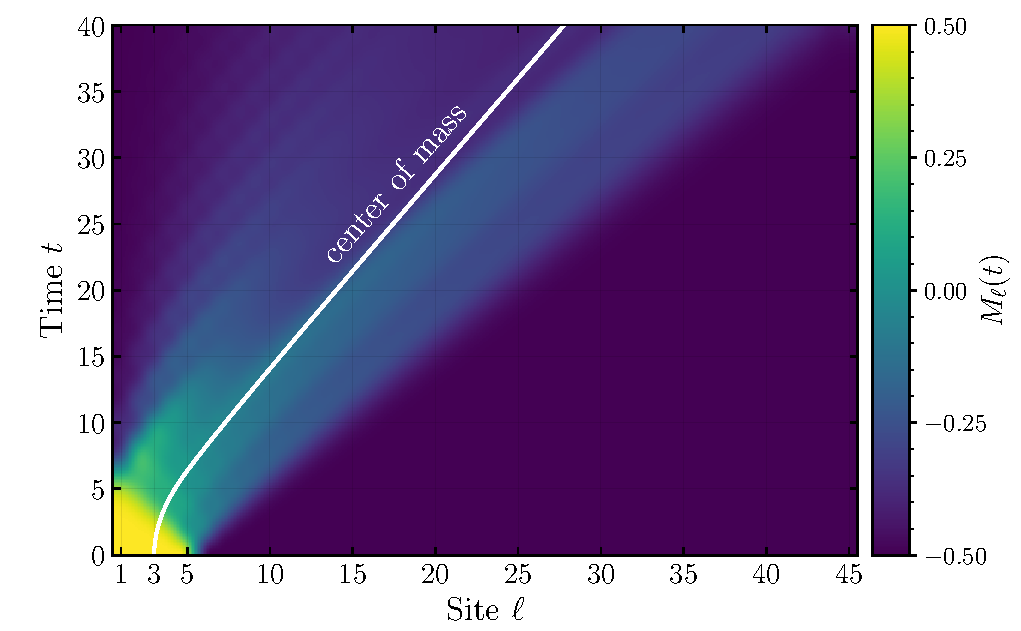
\includegraphics[width=0.8\linewidth]{Figures/magnetization.pdf}
  \caption{Time dependence of magnetization profile \(M_{\ell}(t)\) for \(\alpha = 3.5\) and \(\Delta = 1.0\).
    The evolution of the center of mass, initially at \(r_{\text{cm}}(t=0)=3\), is marked by a white line.}
  \label{fig:magnetization_profile}
\end{figure}
% \newpage
In order to quantitatively investigate the spin transport in this setup, we introduce the so-called
\textbf{center of mass}, defined as the first density moment of the magnetization profile
\begin{equation}
  r_{\text{cm}}(t) = \frac{\sum_{\ell=1}^{L} \ell \left(M_{\ell}(t)+1/2\right)}
  {\sum_{\ell=1}^{L} \left(M_{\ell}(t) + 1/2\right)} =
  \frac{\sum_{\ell=1}^{L} \ell \left(M_{\ell}(t)+1/2\right)}
  {M_{\mathrm{tot}} + L/2}
  \label{eq:center_of_mass}
\end{equation}
In Fig.~\ref{fig:magnetization_profile}, an example of time evolution of center of mass is shown. Examining \(r_{\text{cm}}(t)\)
calculated for two values of \(\Delta = 0.2,\;0.5\) and various values of \(\alpha \in \{2.0,2.5,\ldots,5.0\}\)
(cf. Fig.~\ref{fig:center_of_mass}), we observe a first hint of non-trivial transport properties of the model, namely
non-monotonic dependence of \(r_{\text{cm}}(t)\) on \(\alpha\).

\begin{figure}[htbp]
  \centering
  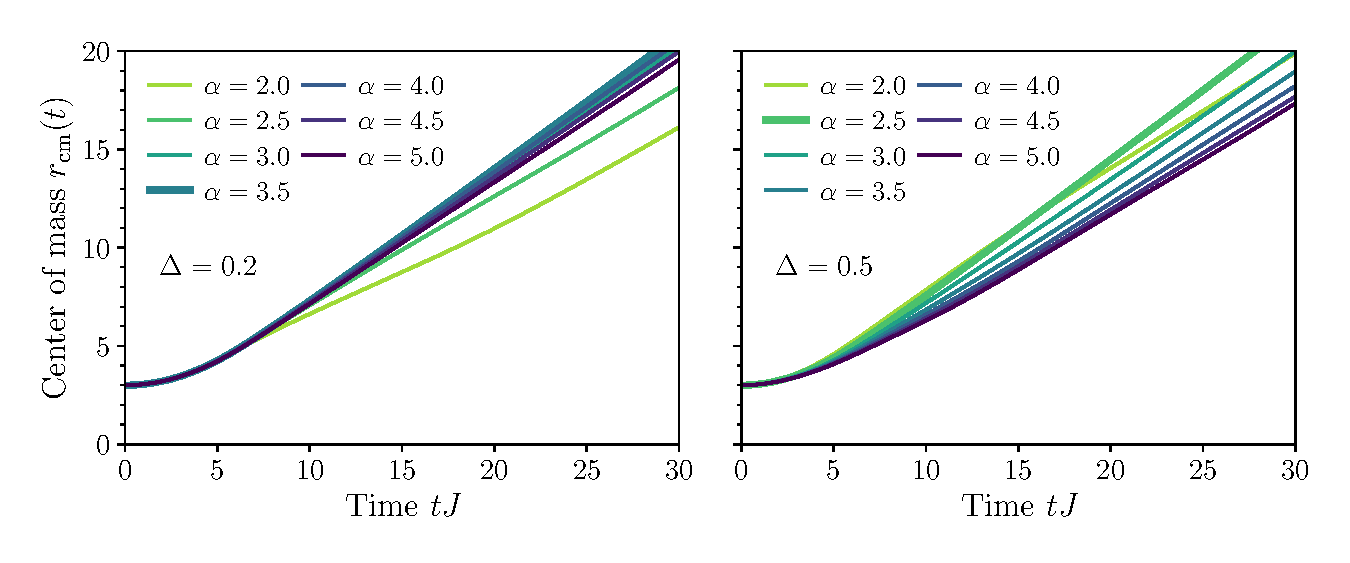
\includegraphics[width=0.9\linewidth]{Figures/center_of_mass.pdf}
  \caption{Time dependence of the center of mass \(r_{\text{cm}}(t)\) for \(\Delta = 0.2\) (left panel) and \(\Delta = 0.5\)
    (right panel) and various values of interaction decay \(\alpha\). The line corresponding to the fastest-moving center of mass
    is thicker than the rest.}
  \label{fig:center_of_mass}
\end{figure}

To see this better, in Fig.~\ref{fig:velocity} we look at the velocity
obtained from the time derivative of the center of mass
\begin{equation}
  {\nu}_{\text{cm}}(t) = \dv{r_{\text{cm}}(t)}{t}.
  \label{eq:velocity}
\end{equation}
\begin{figure}[htbp]
  \centering
  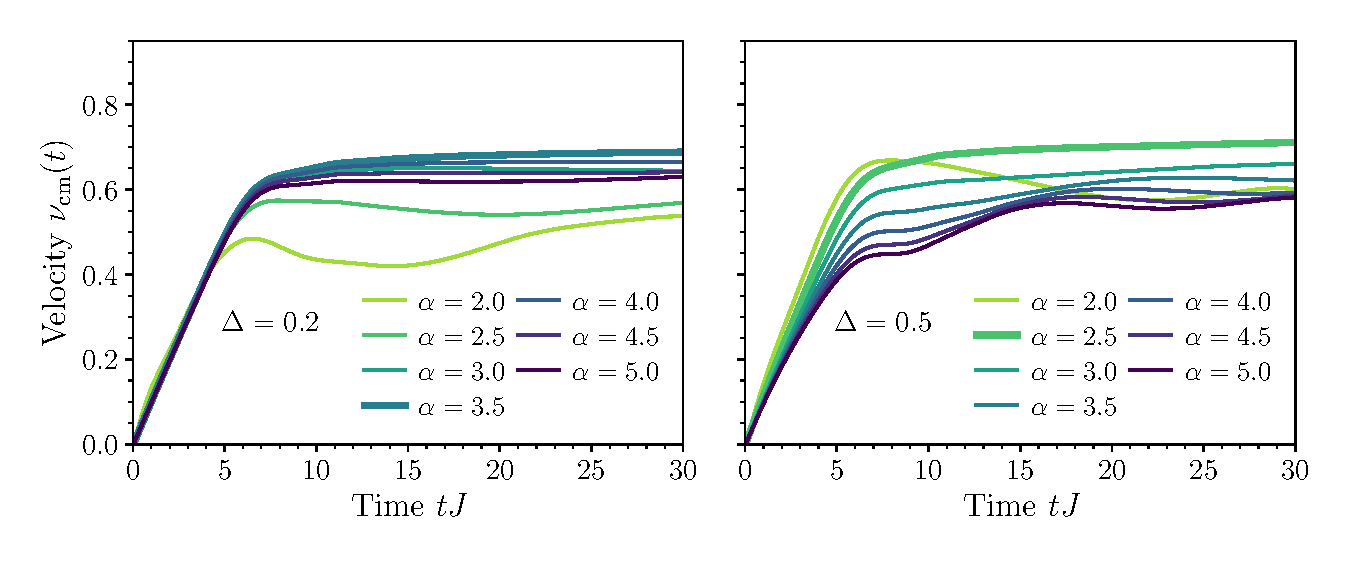
\includegraphics[width=0.9\linewidth]{Figures/velocity.pdf}
  \caption{Time dependence of the velocity \(\nu_{\text{cm}}(t)\) for \(\Delta = 0.2\) (left panel) and \(\Delta = 0.5\)
    (right panel) and various values of interaction decay \(\alpha\). The line corresponding to the largest velocity
    is again thicker than the rest.}
  \label{fig:velocity}
\end{figure}
We observe that for both values of \(\Delta\), there is a clear maximum of the velocity of the expansion
at some intermediate value of \(\alpha\). Investigating further the dependence of velocity on the parameters
of the model, we calculate the average velocity \(\bar{\nu}_{\text{cm}}\) on the interval \(t\in\left[20,30\right]\)
and plot it as a function of \(\alpha\) for various values of \(\Delta\)
(cf. left panel of Fig.~\ref{fig:optimal_velocity}).
The non-monotonic behavior is now evident, as for a fixed \(\Delta\), there exists a value of
\( \alpha = \alpha_{\nu_{\mathrm{max}}}(\Delta) \),
such that the average velocity has a maximum (for \(\Delta = 0.0\) the optimal \(\alpha\) is shifted to infinity).
Equivalently, for each \(\alpha\) there exists an optimal value of \(\Delta = \Delta_{\nu_{\mathrm{max}}} (\alpha)\).

In the right panel of Fig.~\ref{fig:optimal_velocity} we look at the dependence of average velocity on both
parameters of the model. Moreover, we superimpose the points corresponding to the
optimal anisotropies \(\Delta_{\nu_{\mathrm{max}}} (\alpha)\). Curiously, these points
seem to lie very close to an exponential curve, given by \(\Delta_{\mathrm{O}} = \exp\left(-\alpha + 2\right)\).
Furthermore, as seen in the left panel, the average velocity is approximately constant for \(\alpha \geq 2\) and equal to
\(\bar{\nu} \simeq J/\sqrt{2}\) along this line. Such velocity is a characteristic of ballistic
transport in the nearest neighbors free-fermion model~\autocite{Vidmar2013, Langer2012},
corresponding via Jordan-Wigner transformation to our model with \(\alpha \to \infty\) and \(\Delta = 0\).
Therefore, we suspect that the optimal line \(\Delta_{\nu_{\mathrm{max}}} (\alpha)\), present in this interacting
system and indicating \textbf{quasibalistic} transport, is a transient remnant of the transport properties of the free fermions.

\begin{figure}[htbp]
  \centering
  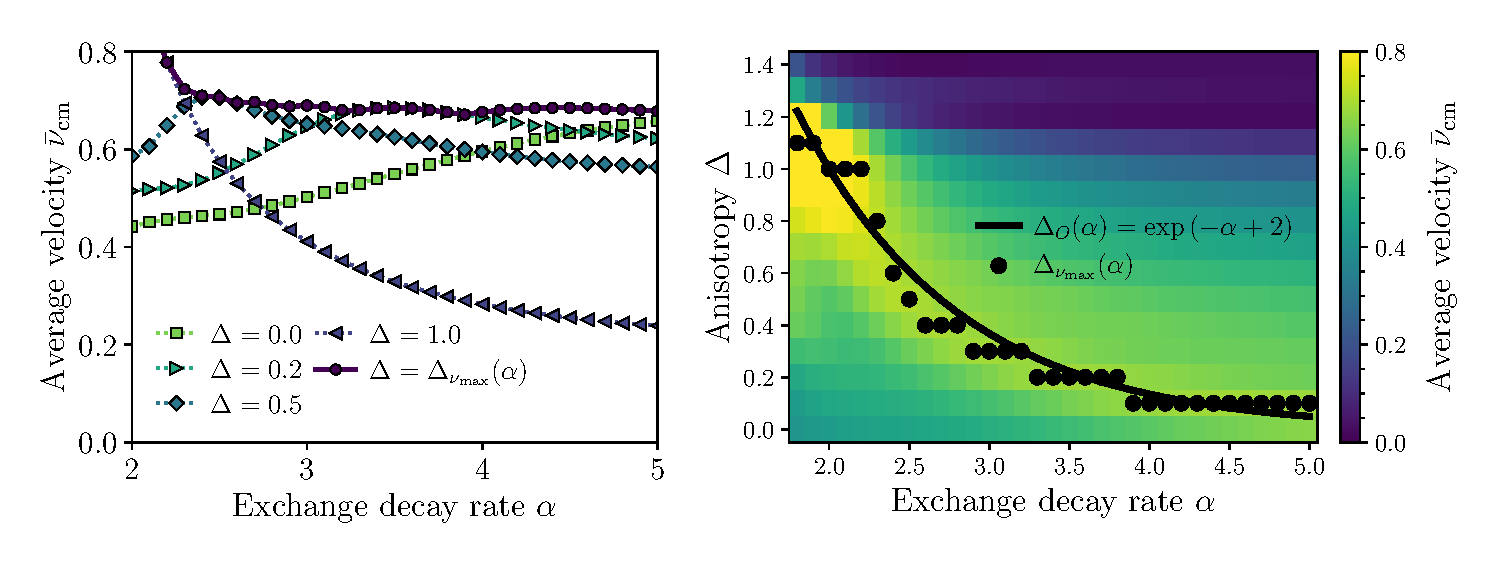
\includegraphics[width=\linewidth]{Figures/optimal_velocity.pdf}
  \caption{Left panel: average velocity \(\bar{\nu}_{\text{cm}}\) as a function of \(\alpha\) for various values of \(\Delta\).
  Right panel: heatmap of the average velocity \(\bar{\nu}_{\text{cm}}\) as a function of \(\alpha\) and \(\Delta\). The points
  corresponding to the optimal anisotropies \(\Delta_{\nu_{\mathrm{max}}} (\alpha)\) are marked with black dots, while the solid line
  indicates the optimal line \(\Delta = \Delta_{\mathrm{O}} = \exp\left(-\alpha + 2\right)\).}
  \label{fig:optimal_velocity}
\end{figure}


\section{Optical conductivity}

In this section, we approach the problem of spin transport in the long-range Heisenberg model from the
perspective of \textbf{linear response theory}. We study the \textbf{optical conductivity}
\footnote{The optical conductivity is also known as the spin conductivity. Technically, as shown in the appendix~\ref{app:opt_cond},
this the \textit{real} part of the optical conductivity, but it is enough to study it as the real part and the imaginary part
are related via the Kramers-Kronig relation.} \(\sigma(\omega)\) of the model,
which is a measure of the response of the system to an external electromagnetic field.
In the linear response regime, the optical conductivity is given by the Kubo formula, which
for infinite temperature reads
\begin{equation}
  \sigma(\omega) = \frac{\pi}{L \mathcal{Z}} \sum_{n,m} \abs{\mel{n}{j^{\sigma}}{m}}^2 \delta(\omega - \epsilon_m + \epsilon_n)
  \label{eq:kubo}
\end{equation}
where \(\mathcal{Z}\) is the number of states in the Hilbert space, \(L\) is the system size and \(j^{\sigma}\) is the spin
current operator~\eqref{eq:spin_current}, derived in Chapter~\ref{chap:intro}.
For the derivation of the Kubo formula and the optical conductivity, see Appendix~\ref{app:opt_cond}.
As the sum in Eq.~\eqref{eq:kubo} runs
uniformly over all many-body eigenstates \(H \ket{n} = \epsilon_n \ket{n}\) of the Hamiltonian, this quantity
probes the whole eigenspectrum. Equation~\ref {eq:kubo} suggests a simple numerical procedure for calculating
the optical conductivity. First, one needs to diagonalize the Hamiltonian \(H\) and obtain the eigenstates
\(\ket{n}\) and eigenvalues \(\epsilon_n\). Then, one needs to calculate the matrix elements of the spin current operator
\(\mel{n}{j^{\sigma}}{n}\) between all pairs of eigenstates. Finally, the optical conductivity is obtained by
summing over all pairs of eigenstates, weighted by the corresponding matrix elements and the \(\delta\) function.
It is only the last step that requires some care, as the \(\delta\) function is not a regular function and
would require some binning of the discrete spectrum. We avoid this, by instead considering the
\textbf{integrated conductivity}
\begin{equation}
  \mathcal{I}(\Omega) = \frac{1}{\mathcal{S}_{\mathrm{tot}}} \int_{-\Omega}^{\Omega} \sigma(\omega) \dd{\omega} =
  \frac{\pi}{L \mathcal{Z} \mathcal{S}_{\mathrm{tot}}} \sum_{n,m} \abs{\mel{n}{j^{\sigma}}{m}}^2 \theta(\Omega- \abs{\epsilon_m - \epsilon_n})
  \label{eq:integrated_conductivity}
\end{equation}
where \(\theta(x)\) is the Heaviside step function and  \(\mathcal{S}_{\mathrm{tot}}\) is the sum rule
\begin{equation}
  \mathcal{S}_{\mathrm{tot}} = \int_{-\infty}^{\infty} \sigma(\omega) \dd{\omega} = \frac{\pi}{L \mathcal{Z}} \sum_{n,m} \abs{\mel{n}{j^{\sigma}}{m}}^2
\end{equation}
It is easy to see that the integrated conductivity \(\mathcal{I}(\Omega)\) is a regular function of \(\Omega\), and
contains the information about the fraction of the spectral weight contained in the frequency window
\(\left[-\Omega,\Omega\right]\).
Equation~\eqref{eq:integrated_conductivity} is now straightforward to evaluate numerically.

We evaluate the integrated conductivity~\eqref{eq:integrated_conductivity} for the long-range Heisenberg model
with periodic boundary conditions, and system sizes up to \(L=20\). We also restrict the calculations to the
subspace of zero total magnetization, i.e. the largest sector with \(\binom{L}{L/2}\) states. Leveraging
the periodic boundary conditions, we perform the calculations separately for each momentum sector and then
add the results together.

\begin{figure}[htbp]
  \centering
  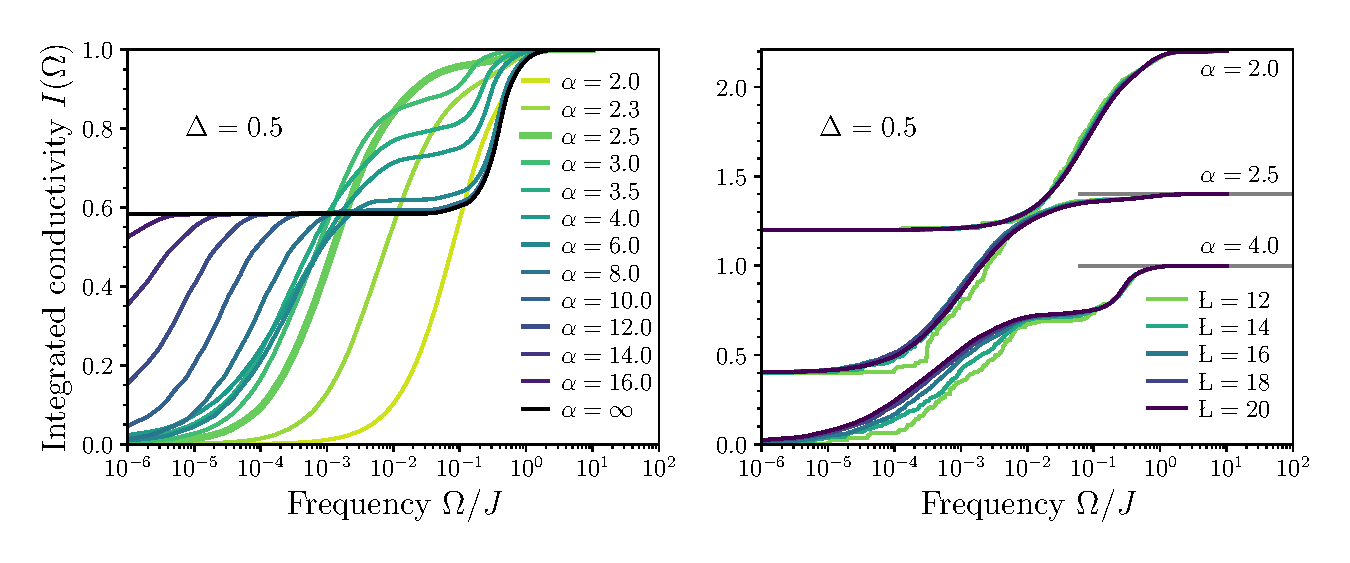
\includegraphics[width=\linewidth]{Figures/optical_conductivity.pdf}
  \caption{Left panel: Integrated conductivity \(\mathcal{I}(\Omega)\) as a function of frequency window \(\Omega\) for various values of \(\alpha\)
    and \(\Delta = 0.5\). The thicker line denotes the result for optimal decay parameter \(\alpha\). Right panel: Size dependence
    of the integrated conductivity \(I(\Omega)\) for \(\alpha = 2.0, \; 2.5,\; 4.0\) and \(\Delta = 0.5\),
    illustrating the effects of finite size. For clarity, we added a vertical shift to distinguish the curves for different
    decay parameters.}
  \label{fig:optical_conductivity}
\end{figure}

Looking at the left panel of Fig.~\ref{fig:optical_conductivity}, we observe that the integrated conductivity
for \(\alpha \to \infty\) is exhibiting a \textbf{Drude peak} behavior at \(\Omega \to 0\), and a distinct
incoherent (regular) spectrum for \(0.1 \lesssim \Omega / J \lesssim 1.0\), which is consistent with the results
for the nearest neighbor Heisenberg model~\autocite{Prelovsek2021}. As \(\alpha\) is decreased
(the range of the interactions increases), but remains \(\alpha \gtrsim 10\), the Drude peak
becomes suppressed, while the regular part of the spectrum is still more or less the same.
However, an interesting feature appears in the spectrum for \(\alpha \lesssim 10\), namely
the incoherent part starts shifting towards lower frequencies. For anisotropy \(\Delta = 0.5\),
this behavior is most pronounced for \(\alpha = 2.5\), where the integrated conductivity
is \(\mathcal{I}(\Omega)\simeq 1 \) for all \( \Omega/J < 0.01\), which means that most of the spectral weight
is contained in the frequency window \(\left[-0.01,0.01\right]\). This in turn implies ballistic-like
spin transport for extremely long times up to \(tJ \simeq 100\), similar to the case of noninteracting particles,
as there we have \(\sigma(\omega) \propto \delta(\omega) \implies I(\Omega) = 1\) for \(\Omega > 0\). Furthermore,
we once again observe some kind of non-monotonic behavior, as decreasing the decay parameter
beyond \(\alpha \approx 2.5\) shifts the incoherent part of the spectrum back towards higher frequencies.

To quantitatively investigate this effect across the parameter space, in Fig.~\ref{fig:I_cond_heatmap}
we present heatmaps of the integrated conductivity \(\mathcal{I}(\Omega)\) on the \((\alpha ,\Omega)\) plane,
for different values of the anisotropy \(\Delta\). Moreover, with a solid black line we denote the
the value \(\Omega = \Omega^{\ast}\), for which the integrated conductivity is \(\mathcal{I}(\Omega^{\ast}) = 0.9\),
i.e. 90\% of the sum rule \(S_{\mathrm{tot}}\).


As in the case of average velocity during a spin expansion experiment,
for every value of \(\Delta\), we can find a value of \(\alpha\) for which the quantity telling about transiency
of ballistic transport admits extremal value. Here, it is the \(\Omega^{\ast}\) that becomes minimal,
and in fact surprisingly small, implying transient ballistic spin transport. Once again, we can proceed
in reverse, and extract the optimal anisotropy \(\Delta_{\sigma} = \Delta_{\sigma}(\alpha)\) as a function
of the decay parameter \(\alpha\), for which \(\Omega^{\ast}\) is minimal. We can thus directly compare
the optimal anisotropies obtained from the two different quantities, namely the average velocity and the integrated conductivity.

\begin{figure}[htbp]
  \centering
  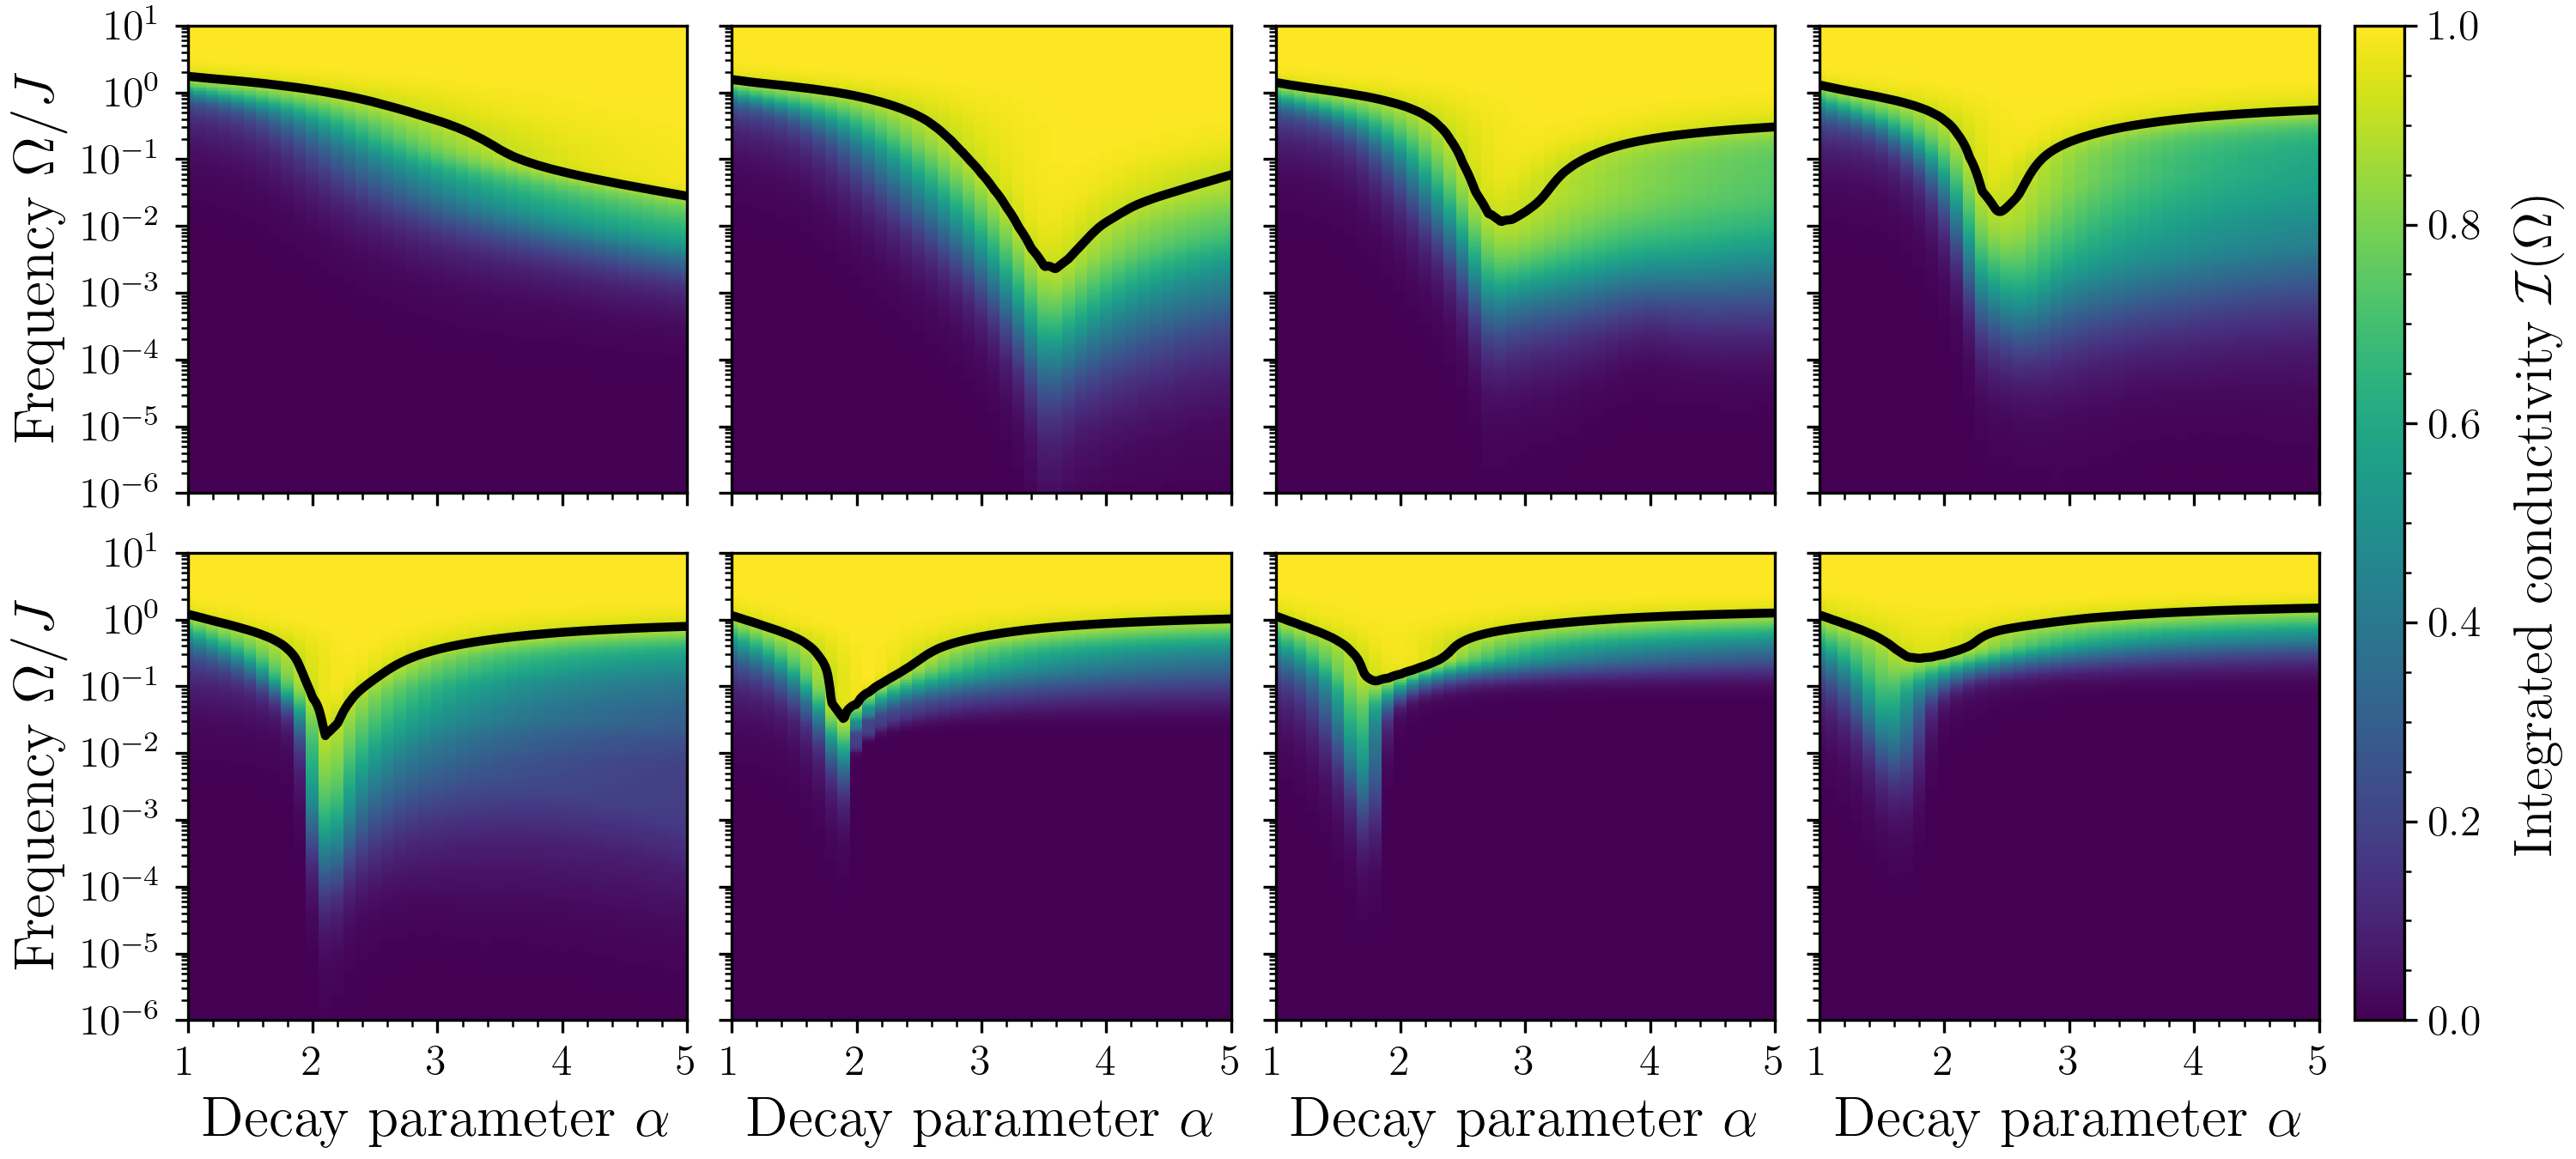
\includegraphics[width=\linewidth]{Figures/I_cond_heatmap.png}
  \caption{Heatmaps of the integrated conductivity \(\mathcal{I}(\Omega)\) on the \((\alpha ,\Omega)\) plane.
    Black solid line denotes the value \(\Omega = \Omega^{\ast}\),
    for which the integrated conductivity is \(I(\Omega^{\ast}) = 0.9\).}
  \label{fig:I_cond_heatmap}
\end{figure}

The results are presented in Fig.~\ref{fig:optimal_anisotropy}, and we observe an excellent
agreement between \(\Delta_{\sigma}\) obtained from linear response theory, that is low frequency (long time) dynamics,
of a system with periodic boundary conditions,
and the optimal anisotropy \(\Delta_{O}(\alpha)\), inferred from the short-time spin domain expansion in a chain
with open boundary conditions. This is a strong indication that the transient ballistic spin transport
is a generic feature of the long-range Heisenberg model, and not an artifact of the finite system size.
It is further supported by the finite-size analysis of the integrated conductivity, presented in the right panel
of Fig.~\ref{fig:optical_conductivity}, where we observe that \(\mathcal{I}(\Omega)\) for \(\alpha = 2.0\)
is almost independent of the system size, and for larger values of \(\alpha\), the incoherent part of the spectrum
is shifted towards even lower frequencies.

\begin{figure}[htbp]
  \centering
  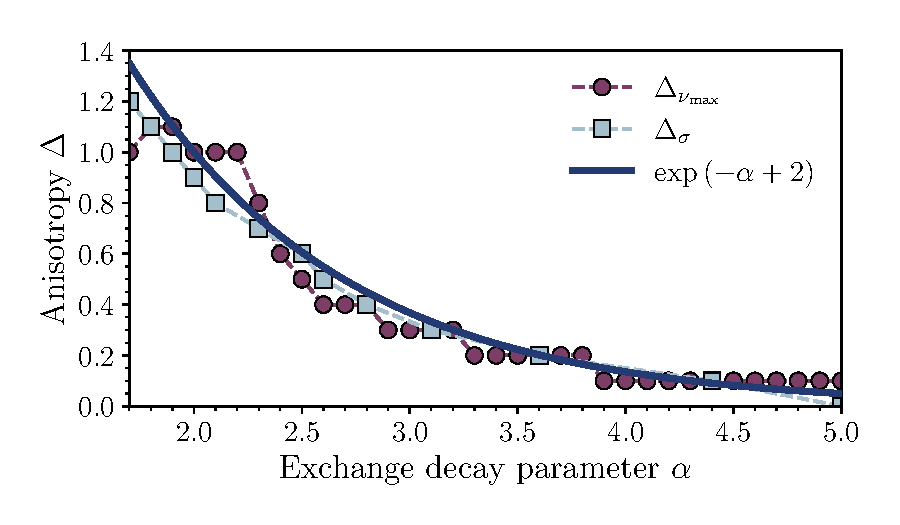
\includegraphics[width=0.8\linewidth]{Figures/optimal_anisotropies.pdf}
  \caption{Optimal values of anisotropy \(\Delta\), as a function of decay parameter \(\alpha\), obtained from
    the average velocity of spin expansion and integrated conductivity. The solid line denotes the optimal line
    \(\Delta_{\mathrm{O}} = \exp\left(-\alpha + 2\right)\).}
  \label{fig:optimal_anisotropy}
\end{figure}


It is worth mentioning, that in~\textcite{Mierzejewski2023},
we have also looked into a generalized version of the aforementioned Haldane-Shastry model,
with the exchange interaction of the form \(J_{\mathrm{HS}(\alpha)} \propto 1/\sin^{\alpha}(\pi r/L)\).
We have shown that it exhibits very similar behavior, with the integrated conductivity
close to the one obtained for the long-range Heisenberg model, and the optimal anisotropy
following the same exponential curve. Moreover, we have investigated two other
models, namely the next-nearest neighbor Heisenberg model (i.e.~\eqref{eq:long_range} with \(r_\mathrm{max} = 2\)),
and the long-range \(t\)-\(V\) spinless fermion model.
Contrary to the nearest-neighbor case, the long-range \(t\)-\(V\) model is not related to the long-range
Heisenberg model via the Jordan-Wigner transformation, and thus the two models are not equivalent.
The former case yielded results similar to the long-range Heisenberg model for small values
of anisotropy \(\Delta\in\left[0,0.2\right]\), while for larger values of \(\Delta\), the integrated conductivity
was rather featureless. It is consistent with our main results, as is this parameter regime, the optimal
decay is \(\alpha \gtrsim 3.5\), rendering the terms with \(r > 2\) insignificant.
In the latter case of spinless fermions, the quasibalistic transport was all but absent. Therefore,
it is expected that this phenomenon is unique to the long-range Heisenberg model.
For more details about those results, that go beyond the scope of this thesis, the interested reader is referred to
the original research article.

\cleardoublepage{}

\chapter{Relaxation eigenmodes in long range XXZ model}
\thispagestyle{chapterBeginStyle}

The results concerning spin transport in the long range XXZ have already been published in~\textcite{Mierzejewski2023}.
\cleardoublepage{}

\chapter{Summary}
\thispagestyle{chapterBeginStyle}


The overarching goal of the work presented in this thesis, serving as the background, is to understand the properties of
quantum systems that are close to integrability, as they facilitate real-world implementation, while
still maintaining some desired properties of strictly integrable systems.
To aid this development, there is a strong need for a robust set of theoretical tools that one
could use for the investigation of such systems. As most of the sophisticated machinery developed
for integrable systems cease to work for the case of nearly integrable systems, one has
to resort to numerical methods. It is impossible to touch upon all the aspects of this
topic in a short thesis, thus we had two concrete goals in mind.

We started with a comprehensive introduction to the numerical methods, beyond the simplest Exact
Diagonalization, that are used in the study of quantum many-body systems. To this end, we presented
the Krylov subspace methods, which are designed to leverage the sparsity of matrix representations of
physical observables, in order to speed up the computations. Starting from the very beginning, we
introduced in detail the Arnoldi iteration, which is most often used to find the extremal eigenvalues
of general, non-Hermitian matrices, even though it does so rather accidentally. We then moved on to
the case of Hermitian matrices, where this procedure reduces to the well-known and versatile
Lanczos iteration. As an immediate application of the Lanczos iteration, beyond just the ground state
computations, the so-called Krylov propagator was presented, which allows one to compute the time evolution of
a state vector, without the need for diagonalization of the Hamiltonian. Finally, we described,
and partially derived, an approach to the correlation functions, based on the Krylov
propagator and the concept of Quantum Typicality, which allows one to compute them
without explicitly carrying out the trace over all many-body states.

The main goal was to apply those methods to the study of the dynamics of the spin transport in the anisotropic
Heisenberg model with power-law interaction \(J(\alpha) = J/r^{\alpha}\), which is an important example of a
long-range interacting system. Motivated by experimental setups, we started by considering the
expansion of a domain-wall initial state and found a non-monotonic dependence of the
center of mass velocity on the anisotropy parameter. By considering maximal velocities,
we found a line in the parameter space, \(\Delta_O(\alpha) = \exp(-\alpha + 2)\),
for which the velocity of spin domain wall expansion is similar to the case of free
nearest-neighbors particles, indicating short-time (high-frequency) ballistic transport.
Next, we studied spin transport from the perspective of the linear response theory,
by considering the optical conductivity and its integral over a frequency window.
It revealed a regime of quasi-ballistic transport, where the spectral sum
of the optical conductivity accumulated at frequencies below \(\Omega^{\ast}/J \sim
10^{-3}-10^{-2}\). As a result, along the line of optimal anisotropy, the spin
transport is ballistic for surprisingly long times, up to \(t \sim 1/\Omega^{\ast}\),
which is in agreement with the results of the domain-wall expansion. The entirety of
the results presented in Chapter~\ref{chap:spin_transport} were obtained by the coauthors of~\textcite{Mierzejewski2023}.
We also investigated the properties of local, slowly relaxing observables
(LSROs), obtained using a numerical algorithm designed to find local integrals of
motion in integrable systems. For completeness, we provided a rather detailed
description of the algorithm itself, together with a possible upgrade, replacing
ED-based time averaging with Lanczos-based long-time correlation functions.
Unfortunately, the upgraded approach turned out to be unsuitable for the purpose of
this thesis, as matrices of long-range operators are no longer sparse and thus do not
benefit from the Lanczos iteration. Nevertheless, using the original algorithm, we
found that the best LSROs decay the slowest precisely for the optimal anisotropy, obtained from
previous methods. Additionally, we showed that they can be understood in terms of projections onto
current-like operators, corresponding via the Jordan-Wigner transformation to long-range fermionic hoppings,
even though the Hamiltonian does not admit a representation in terms of two-body fermionic operators.
Finally, using the finite-time averaging version of the algorithm, we investigated the frequency dependence
of the LSROs, akin to the optical conductivity, and found that the concentration of the spectral weight
resembles the one of the optical conductivity. Chapter~\ref{chap:currents} contains the original work
of the author of this manuscript.

The main result of this thesis, and the broader research published in \textcite{Mierzejewski2023}, is the
discovery of the line of optimal anisotropy, \(\Delta_{\mathrm{O}}(\alpha) = \exp(-\alpha +2)\),
along which the spin transport is ballistic for surprisingly long times \(tJ \sim 10^{-2} -10^{-3}\).
This line smoothly interpolates between integrable two models with purely ballistic
transport, namely free particles for \(\alpha =\infty,\; \Delta =0\) and Haldane-Shastry
like model for \(\alpha  = 2,\; \Delta  = 1\). It suggests that the long-range Heisenberg
model can be thought of as nearly-integrable far beyond just the vicinity of the
integrable limits, but rather for a whole line of parameters. Unfortunately, the precise
microscopic origin of the optimal anisotropy is still unknown. A possible explanation
would be that for \(\delta = \exp(-\alpha  + 2)\) this model is very close to some,
more complicated, integrable model, in which the spin current is an integral of motion.
Investigation of systems similar to the one studied in this thesis, from the perspective
of the search for remnants of integrability, is a promising direction for future research.

\cleardoublepage{}

%%%%%%%%%%%%%%%%%%%%%%%%%%%%%%%%%%%%%%%%%%%%%%%%%%%%%%%%%%%%%%%%%%%%%%%%%%%%%%
%%%%%%%%%%%%%%%%%%%%%%%%%%%%%%% BIBLIOGRAFIA %%%%%%%%%%%%%%%%%%%%%%%%%%%%%%%%%
%%%%%%%%%%%%%%%%%%%%%%%%%%%%%%%%%%%%%%%%%%%%%%%%%%%%%%%%%%%%%%%%%%%%%%%%%%%%%%

\pagestyle{bibliographyStyle}
\printbibliography{}
\thispagestyle{chapterBeginStyle}
\addcontentsline{toc}{chapter}{Bibliography}
\cleardoublepage{}

%%%%%%%%%%%%%%%%%%%%%%%%%%%%%%%%%%%%%%%%%%%%%%%%%%%%%%%%%%%%%%%%%%%%%%%%%%%%%%
%%%%%%%%%%%%%%%%%%%%%%%%%%%%%%%%% DODATKI %%%%%%%%%%%%%%%%%%%%%%%%%%%%%%%%%%%%
%%%%%%%%%%%%%%%%%%%%%%%%%%%%%%%%%%%%%%%%%%%%%%%%%%%%%%%%%%%%%%%%%%%%%%%%%%%%%%

\appendix
\pagestyle{appendixStyle}
\chapter{Hilbert subspaces with fixed momentum\label{app:momentum}}
\thispagestyle{chapterBeginStyle}

\cleardoublepage{}

\end{document}

